% study_guide.tex — how the stfu codebase works
%
% Build:  cd docs && latexmk -pdf study_guide.tex      (pdflatex, bare TeX Live is enough)
%    or:  pdflatex study_guide && pdflatex study_guide  (twice, for the table of contents)
%
% Every diagram is TikZ drawn inline, so there are no image files to keep in sync.
% Sections point to source files with \file{...}; readers are expected to open the file
% alongside the text.

\documentclass[10pt,a4paper]{article}

\usepackage[T1]{fontenc}
\usepackage[utf8]{inputenc}
\usepackage{lmodern}
\usepackage{microtype}
\usepackage[htt]{hyphenat}
\usepackage[margin=2.2cm,headheight=14pt]{geometry}
\usepackage{xcolor}
\usepackage{tikz}
\usepackage{pgfplots}
\pgfplotsset{compat=1.18}
\usepgfplotslibrary{fillbetween}
\usetikzlibrary{arrows.meta,positioning,fit,backgrounds,calc,shapes.geometric,
  shapes.multipart,decorations.pathreplacing,automata,matrix,patterns,quotes}
\usepackage{booktabs}
\usepackage{tabularx}
\usepackage{longtable}
\usepackage{multicol}
\usepackage{array}
\usepackage{enumitem}
\usepackage{caption}
\usepackage{titlesec}
\usepackage{fancyhdr}
\usepackage{amsmath,amssymb}
\usepackage[most]{tcolorbox}
\usepackage[hidelinks,bookmarksnumbered]{hyperref}
\usepackage{cleveref}

% ----------------------------------------------------------------- colours ---
% The app's own palette: deep teal and mint (see ui/theme/Color.kt and the launcher icon).
\definecolor{teal}{HTML}{0F4C5C}
\definecolor{mint}{HTML}{7FE0C3}
\definecolor{amber}{HTML}{E09F3E}
\definecolor{rust}{HTML}{9E2A2B}
\definecolor{slate}{HTML}{5C677D}
\definecolor{paper}{HTML}{F4F6F5}
% One colour per workload, used consistently in every diagram.
\definecolor{wa}{HTML}{2A9D8F}   % A sensing & service
\definecolor{wb}{HTML}{E76F51}   % B signal & calibration
\definecolor{wc}{HTML}{8E7DBE}   % C notifications
\definecolor{wd}{HTML}{F4A261}   % D UI & stats
\definecolor{ws}{HTML}{6C757D}   % shared core

% ------------------------------------------------------------------ macros ---
\newcommand{\file}[1]{\texttt{\small #1}}          % a source file the reader should open
\newcommand{\code}[1]{\texttt{#1}}                  % a symbol: class, function, field
\newcommand{\wl}[1]{\textbf{Workload #1}}
\newcommand{\state}[1]{\textsc{\small #1}}          % FOCUSED, NOT_FOCUSED, UNKNOWN
\newcommand{\Thigh}{T_{\mathrm{high}}}
\newcommand{\Tlow}{T_{\mathrm{low}}}
\newcommand{\uV}{\textmu V\textsuperscript{2}}

% "Open these files" box at the start of each section.
\newtcolorbox{files}{enhanced,colback=paper,colframe=slate!60,boxrule=0.5pt,
  arc=1.5pt,left=6pt,right=6pt,top=4pt,bottom=4pt,fontupper=\small,
  title=\textsc{Files to read alongside this section},coltitle=white,colbacktitle=slate!80}
% Short "why" notes that a question in the oral exam is likely to probe.
\newtcolorbox{why}[1][]{enhanced,colback=teal!4,colframe=teal,boxrule=0.6pt,arc=1.5pt,
  left=6pt,right=6pt,top=4pt,bottom=4pt,title={#1},fonttitle=\bfseries\small}
% Something that was broken, or a known limit worth being able to describe honestly.
\newtcolorbox{gotcha}[1][]{enhanced,colback=amber!8,colframe=amber!80!black,boxrule=0.6pt,
  arc=1.5pt,left=6pt,right=6pt,top=4pt,bottom=4pt,title={#1},fonttitle=\bfseries\small}
% Question bank entries.
\newcounter{qnum}
\newcommand{\Q}[2]{\stepcounter{qnum}\par\medskip\noindent
  \textbf{Q\theqnum.}\ #1\par\nobreak\smallskip\noindent
  {\color{teal}\textbf{A.}}\ #2\par}

% ------------------------------------------------------------------ layout ---
\titleformat{\section}{\Large\bfseries\color{teal}}{\thesection}{0.8em}{}
\titleformat{\subsection}{\large\bfseries\color{teal!80!black}}{\thesubsection}{0.7em}{}
\titleformat{\subsubsection}{\normalsize\bfseries}{\thesubsubsection}{0.6em}{}
\titlespacing*{\section}{0pt}{2.2ex plus 1ex minus .2ex}{1.4ex plus .2ex}
\setlist{nosep,leftmargin=*}
\captionsetup{font=small,labelfont={bf,color=teal},width=0.92\linewidth}
\pagestyle{fancy}
\fancyhf{}
\fancyhead[L]{\small\textsc{stfu} \textperiodcentered\ how the code works}
\fancyhead[R]{\small\nouppercase{\leftmark}}
\fancyfoot[C]{\small\thepage}
\renewcommand{\headrulewidth}{0.3pt}
\setlength{\parskip}{0.35em}
\setlength{\parindent}{0pt}
\renewcommand{\arraystretch}{1.15}

% TikZ styles shared by every diagram.
\tikzset{
  >={Latex[length=2.2mm,width=1.8mm]},
  box/.style={draw=slate!70,rounded corners=2pt,fill=white,align=center,font=\small,
    minimum height=8mm,inner sep=4pt},
  wabox/.style={box,fill=wa!22,draw=wa!80!black},
  wbbox/.style={box,fill=wb!22,draw=wb!80!black},
  wcbox/.style={box,fill=wc!22,draw=wc!80!black},
  wdbox/.style={box,fill=wd!25,draw=wd!80!black},
  wsbox/.style={box,fill=ws!15,draw=ws},
  iface/.style={draw=teal,dashed,rounded corners=2pt,fill=teal!6,align=center,
    font=\small\ttfamily,minimum height=8mm,inner sep=4pt},
  ext/.style={box,fill=paper,draw=slate,font=\small\itshape},
  flow/.style={->,thick,color=slate!90!black},
  note/.style={font=\footnotesize\itshape,color=slate!90!black,align=center},
  lbl/.style={font=\footnotesize,color=black,align=center,fill=white,inner sep=1.5pt},
  st/.style={draw=teal,thick,circle,fill=teal!8,minimum size=16mm,align=center,font=\small\scshape},
}

\hypersetup{pdftitle={stfu: how the code works},pdfauthor={COMPX551 group}}

\begin{document}

% ------------------------------------------------------------- title page ---
\begin{titlepage}
\centering
\vspace*{2.5cm}
{\color{teal}\rule{\textwidth}{1.2pt}}\par\vspace{0.6cm}
{\Huge\bfseries\color{teal} stfu}\par\vspace{0.3cm}
{\LARGE How the code works}\par\vspace{0.5cm}
{\large A study guide to the focus-aware notification deferral app}\par
\vspace{0.6cm}{\color{teal}\rule{\textwidth}{1.2pt}}\par
\vspace{1.2cm}
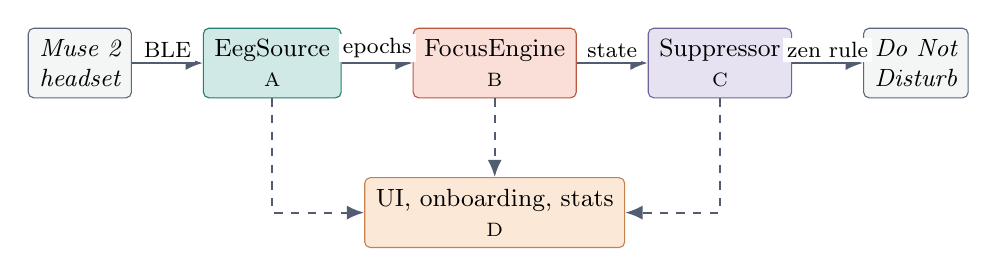
\begin{tikzpicture}[node distance=5mm and 9mm]
  \node[ext](muse){Muse 2\\headset};
  \node[wabox,right=of muse](src){EegSource\\\scriptsize A};
  \node[wbbox,right=of src](eng){FocusEngine\\\scriptsize B};
  \node[wcbox,right=of eng](sup){Suppressor\\\scriptsize C};
  \node[ext,right=of sup](dnd){Do Not\\Disturb};
  \node[wdbox,below=10mm of eng](ui){UI, onboarding, stats\\\scriptsize D};
  \draw[flow](muse)--(src) node[midway,above,lbl]{BLE};
  \draw[flow](src)--(eng) node[midway,above,lbl]{epochs};
  \draw[flow](eng)--(sup) node[midway,above,lbl]{state};
  \draw[flow](sup)--(dnd) node[midway,above,lbl]{zen rule};
  \draw[flow,dashed](src.south)|-(ui.west);
  \draw[flow,dashed](sup.south)|-(ui.east);
  \draw[flow,dashed](eng)--(ui);
\end{tikzpicture}
\vfill
\begin{minipage}{0.8\textwidth}\small
\textbf{Purpose.} Written for the team's internal review before the oral examination. A reader who
works through it, with the named source files open beside it, should be able to explain how any
part of the app works, why it is built that way, and what its known limits are. Harder parts of
the code get more space than easy ones.\par\medskip
\textbf{Code state.} Describes \code{main} at commit \code{bf5774e} (3 October 2026), about
9{,}900 lines of Kotlin, plus the \code{FocusService} scope fix made while writing this guide.
Line references are to that commit and will drift as files change.
\end{minipage}
\vspace{1cm}
\par{\small COMPX551 \textperiodcentered\ Assignment 4 \textperiodcentered\ October 2026}
\end{titlepage}

\begin{multicols}{2}\small\tableofcontents\end{multicols}
\clearpage
% =============================================================================
\section{How to use this guide}
% =============================================================================

The app has one job: while a Muse EEG headset says the wearer is concentrating, hold their
phone's notifications back, and when concentration breaks, deliver what was held as one quiet
summary. Everything in the codebase serves that sentence, and the oral exam will probe whether
you can trace any feature back to it.

\paragraph{Reading order.} \Cref{sec:architecture} explains the shape of the whole thing and the
six interfaces that hold it together; read it first regardless of which workload you own. The
four workload sections (\cref{sec:a,sec:b,sec:c,sec:d}) then go through each area. The length of
each is proportional to how hard it is to explain under questioning, not to how many lines it has:
the signal path in \cref{sec:b} gets the most room because it carries the most numbers, and
the notification layer gets more than its line count suggests because its behaviour is mostly
dictated by Android rules that are easy to misstate. \Cref{sec:integration} covers what changed
when the four branches were merged, which matters because several of those changes alter
behaviour that a workload owner may still describe the old way. \Cref{sec:questions} is a question
bank with answers.

\paragraph{Files.} Each section opens with a box naming the source files it describes. The text
does not reproduce the code. Open the file, find the function named in the text, and read it
against the explanation; that pairing is what the guide is designed for. Line numbers are given
as \code{path:line} and refer to commit \code{bf5774e}.

\paragraph{Conventions.} Workloads are colour-coded in every diagram:
\tikz[baseline=-0.6ex]\node[wabox,minimum height=4mm,inner sep=2pt,font=\scriptsize]{A};\ sensing and service,
\tikz[baseline=-0.6ex]\node[wbbox,minimum height=4mm,inner sep=2pt,font=\scriptsize]{B};\ signal and calibration,
\tikz[baseline=-0.6ex]\node[wcbox,minimum height=4mm,inner sep=2pt,font=\scriptsize]{C};\ notifications,
\tikz[baseline=-0.6ex]\node[wdbox,minimum height=4mm,inner sep=2pt,font=\scriptsize]{D};\ UI and stats,
\tikz[baseline=-0.6ex]\node[wsbox,minimum height=4mm,inner sep=2pt,font=\scriptsize]{S};\ shared core.
Dashed teal boxes are interfaces from \file{core/Contracts.kt}. Focus states are set as
\state{focused}, \state{not\_focused} and \state{unknown}.

% =============================================================================
\section{The system in one picture}\label{sec:architecture}
% =============================================================================

\begin{files}
\file{core/Contracts.kt}, \file{core/Models.kt}, \file{AppContainer.kt},
\file{app/src/main/AndroidManifest.xml}, \file{DESIGN.md}, \file{WORKLOADS.md}
\end{files}

\subsection{Four workloads, one seam}

The project was split four ways before any feature code existed, and the split is visible in the
package layout. \file{WORKLOADS.md} assigns every file to exactly one owner, and the rule was
that nobody edits another person's files. The only coupling between owners is the set of
interfaces in \file{core/Contracts.kt} and the data classes in \file{core/Models.kt}, both
written together in ``sprint 0'' and then frozen. \Cref{fig:workloads} shows the result.

\begin{figure}[htbp]\centering
\resizebox{\textwidth}{!}{%
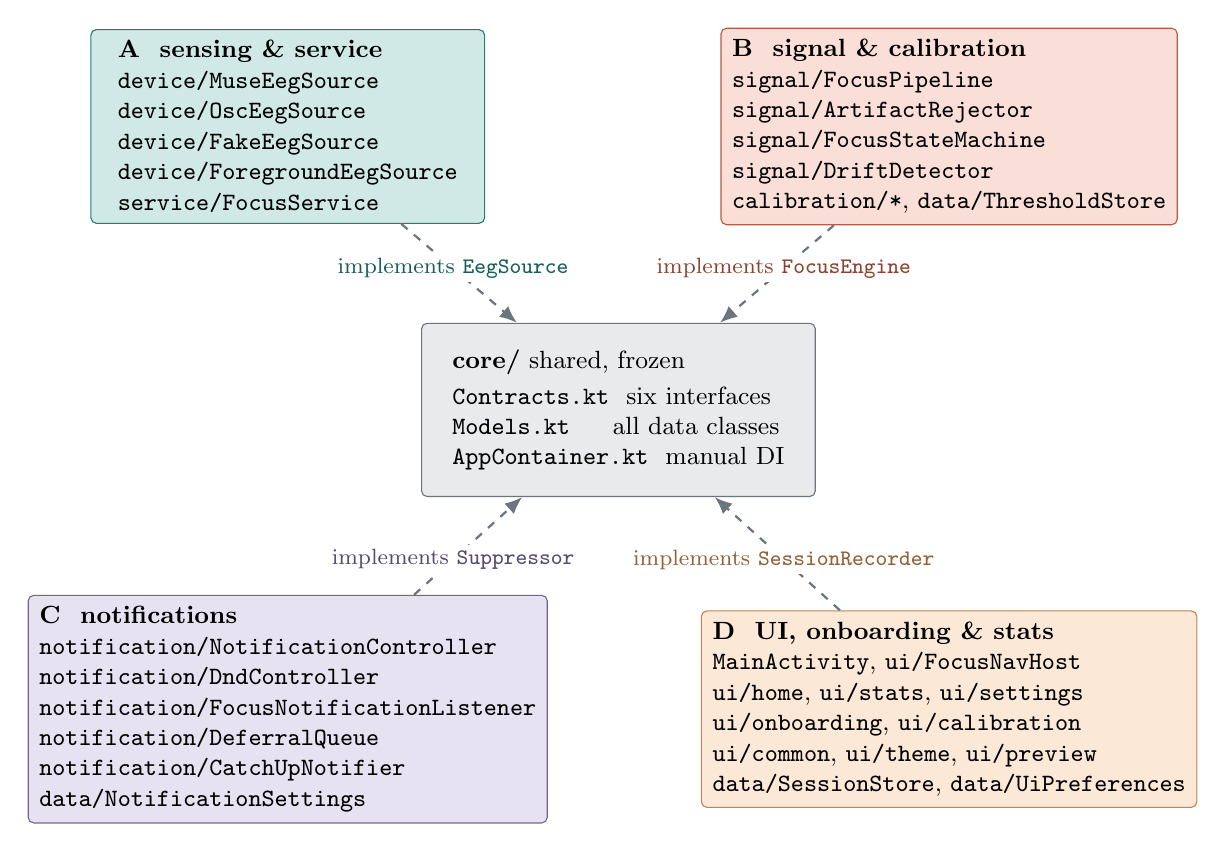
\begin{tikzpicture}[font=\small]
  \node[wsbox,minimum width=50mm,minimum height=22mm,align=left] at (0,0)
    (core) {\textbf{core/} \hfill shared, frozen\\[2pt]
      \texttt{Contracts.kt} \ six interfaces\\
      \texttt{Models.kt} \ \ \ \ all data classes\\
      \texttt{AppContainer.kt} \ manual DI};
  \node[wabox,minimum width=50mm,align=left] at (-4.2,3.6)
    (A) {\textbf{A \ sensing \& service}\\
      \texttt{device/MuseEegSource}\\\texttt{device/OscEegSource}\\
      \texttt{device/FakeEegSource}\\\texttt{device/ForegroundEegSource}\\
      \texttt{service/FocusService}};
  \node[wbbox,minimum width=50mm,align=left] at (4.2,3.6)
    (B) {\textbf{B \ signal \& calibration}\\
      \texttt{signal/FocusPipeline}\\\texttt{signal/ArtifactRejector}\\
      \texttt{signal/FocusStateMachine}\\\texttt{signal/DriftDetector}\\
      \texttt{calibration/*}, \texttt{data/ThresholdStore}};
  \node[wcbox,minimum width=50mm,align=left] at (-4.2,-3.8)
    (C) {\textbf{C \ notifications}\\
      \texttt{notification/NotificationController}\\\texttt{notification/DndController}\\
      \texttt{notification/FocusNotificationListener}\\\texttt{notification/DeferralQueue}\\
      \texttt{notification/CatchUpNotifier}\\\texttt{data/NotificationSettings}};
  \node[wdbox,minimum width=50mm,align=left] at (4.2,-3.8)
    (D) {\textbf{D \ UI, onboarding \& stats}\\
      \texttt{MainActivity}, \texttt{ui/FocusNavHost}\\
      \texttt{ui/home}, \texttt{ui/stats}, \texttt{ui/settings}\\
      \texttt{ui/onboarding}, \texttt{ui/calibration}\\
      \texttt{ui/common}, \texttt{ui/theme}, \texttt{ui/preview}\\
      \texttt{data/SessionStore}, \texttt{data/UiPreferences}};
  \foreach \w in {A,B,C,D} \draw[flow,ws,dashed] (\w) -- (core);
  \node[lbl,text=wa!60!black] at ($(A)!0.5!(core)$) {implements \texttt{EegSource}};
  \node[lbl,text=wb!60!black] at ($(B)!0.5!(core)$) {implements \texttt{FocusEngine}};
  \node[lbl,text=wc!60!black] at ($(C)!0.5!(core)$) {implements \texttt{Suppressor}};
  \node[lbl,text=wd!60!black] at ($(D)!0.5!(core)$) {implements \texttt{SessionRecorder}};
\end{tikzpicture}}
\caption{The package layout mirrors the workload split. Each workload implements one of the four
original interfaces; the two later additions (\code{ServiceController}, \code{NotificationPolicy})
are owned by A and C respectively.}\label{fig:workloads}
\end{figure}

\subsection{The six contracts}

\file{core/Contracts.kt} is 122 lines and is the single most important file to know cold. The
four original interfaces follow the data path, and two more were added by D during sprint~0
because the UI needed a master switch and a settings surface (the file's header flags them
``for ratification'').

\begin{table}[htbp]\centering\small
\begin{tabularx}{\textwidth}{@{}l l l X@{}}
\toprule
\textbf{Interface} & \textbf{Owner} & \textbf{Used by} & \textbf{What it promises} \\
\midrule
\code{EegSource} & A & B, D & \code{status: StateFlow<DeviceStatus>}, \code{epochs: Flow<FocusEpoch>}
  at about 1\,Hz. Emits invalid epochs rather than dropping them, so consumers can tell ``bad data''
  from ``no data''. \\
\code{FocusEngine} & B & A, C, D & \code{submit(epoch)} in, \code{state}, \code{decisions} and
  \code{thresholds} out. \code{thresholds} is \code{null} until calibrated and consumers must then
  fail open. Also \code{reset()}, \code{updateThresholds}, \code{fitCalibration},
  \code{recalibrationSuggested}. \\
\code{Suppressor} & C & A & \code{apply(state)} about once a second, so it must be idempotent and
  only touch the platform on a change. \code{flush(reason)} releases the queue as one grouped
  summary. Must fail open on \state{unknown}. \\
\code{SessionRecorder} & D & A, C & Session start/end, every decision, every deferral, every
  flush. Called at 1\,Hz from the service scope, so implementations batch their I/O. \\
\code{ServiceController} & A & D & \code{running} and \code{appliedState}, plus \code{start()} and
  \code{stop()}. The UI must not start the service with a raw Intent because it needs to observe
  whether the service survived Doze. \\
\code{NotificationPolicy} & C & D & \code{settings: StateFlow<PolicySettings>} and
  \code{update()}. Backs the notification section of Settings. \\
\bottomrule
\end{tabularx}
\caption{The six interfaces in \file{core/Contracts.kt}.}\label{tab:contracts}
\end{table}

\begin{why}[Why \code{appliedState} exists alongside \code{FocusEngine.state}]
The engine's state is what the signal says. The applied state is what the suppressor is actually
doing, which differs during the 10\,s signal-loss grace period and whenever the service is not
running. The home screen's status pill shows the applied state so it never disagrees with the
Do Not Disturb rule. This member was added during integration; see \cref{sec:integration}.
\end{why}

\subsection{The data classes}

\file{core/Models.kt} holds every type that crosses a workload boundary. The ones to be able to
describe without looking:

\begin{description}[style=nextline,leftmargin=1.2em]
\item[\code{BandPowers}] Four doubles already reduced from LibMuse's per-channel packets:
  \code{alphaTemporal}, \code{beta1320}, \code{theta}, \code{emgBroadband}. The field names encode
  the design constraints from \file{DESIGN.md}~\S1: alpha from the temporal pair TP9/TP10 because
  it is less eye-contaminated than the frontal pair, and beta clamped to 13--20\,Hz because at a
  forehead electrode 13--30\,Hz is substantially frontalis and temporalis muscle. The computed
  property \code{engagementIndex} is the Pope et al.\ (1995) index
  $\beta/(\alpha+\theta)$.
\item[\code{ContactQuality}] Horseshoe indicator (HSI) per electrode, 1 good to 4 no contact.
  \code{allGood} requires every electrode to be exactly 1.
\item[\code{ArtifactFlags}] One boolean per rejection rule: blink, jaw clench, movement, broadband
  EMG.
\item[\code{FocusEpoch}] One analysis window: timestamp, \code{focusIndex}, \code{bands},
  \code{contact}, \code{artifacts}, and \code{valid}. Invalid epochs are still emitted so the UI
  can draw a gap instead of interpolating.
\item[\code{FocusState}] \state{unknown}, \state{focused}, \state{not\_focused}. \state{unknown}
  means ``no usable signal'' and always means suppression is off.
\item[\code{FocusDecision}] The engine's output per epoch: \code{state}, \code{rawIndex},
  \code{normalizedZ}, \code{accepted}. When \code{accepted} is false the epoch fed no decision and
  \code{normalizedZ} is meaningless.
\item[\code{FocusThresholds}] $\Thigh$ and $\Tlow$ as z-scores, \code{entryDwellSec},
  \code{exitDwellSec}, \code{fittedAtMs}, \code{auc}. The \code{PLACEHOLDER} set, never fitted to
  anyone, is $+0.5$, $-0.2$, 10\,s and 60\,s.
\item[\code{CalibrationBlock}, \code{TaskScore}, \code{CalibrationResult}] The B/D seam. D's
  task screens produce blocks with a \code{TaskScore}; B's fitter consumes them and returns a
  result whose \code{fitted} flag distinguishes ``not enough clean data'' from ``poor separation''.
\item[\code{DeferredNotification}, \code{FlushReason}, \code{PolicySettings}] The notification
  side. \code{FlushReason} has five values so the stats screen can tell the safety valves apart:
  \code{FOCUS\_BROKE}, \code{MAX\_HOLD\_EXCEEDED}, \code{HEADSET\_REMOVED}, \code{SERVICE\_STOPPED},
  \code{MANUAL}.
\item[\code{DeviceState}, \code{DeviceStatus}] Connection state plus battery and contact.
  \code{usable} is true only for \code{CONNECTED}; \code{POOR\_CONTACT} is connected but not
  trustworthy.
\item[\code{SessionSummary}, \code{SessionStats}] What the stats screen renders. Focused time is
  kept per session as a 24-slot by-hour list so the time-of-day pattern survives deleting old
  sessions.
\end{description}

\begin{why}[Why thresholds are z-scores and never raw \uV]
Absolute band power drifts with electrode placement, hair, skin moisture, headband tension, time
of day and caffeine. A raw number calibrated on Tuesday is wrong on Thursday. Storing z-scores
makes the thresholds relative to a distribution, and the pipeline's job becomes supplying the
right distribution to score against (\cref{sec:b:pipeline}).
\end{why}

\subsection{The runtime data path}

\Cref{fig:dataflow} is the picture to have in your head when answering any ``what happens
when\ldots'' question. The headset produces samples at 256\,Hz; LibMuse reduces them to band
powers; the source reduces those to one \code{FocusEpoch} per second; the engine turns epochs
into a state; the suppressor turns state changes into Do Not Disturb toggles; and the recorder
logs the lot for the stats screen. The whole chain runs inside \code{FocusService}'s coroutine
scope regardless of whether any screen is open.

\begin{figure}[htbp]\centering
\resizebox{\textwidth}{!}{%
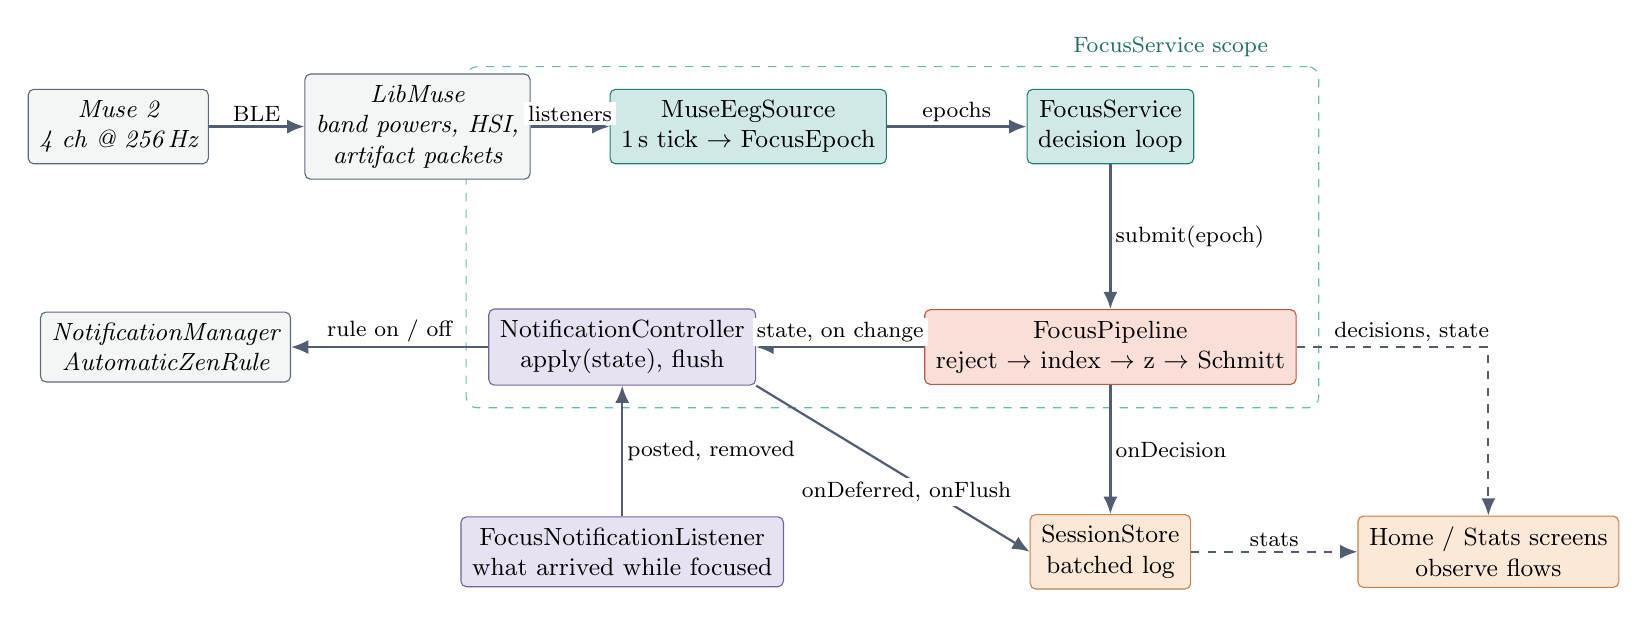
\begin{tikzpicture}[font=\small]
  \node[ext]   at (0,0)    (muse){Muse 2\\4 ch @ 256\,Hz};
  \node[ext]   at (3.8,0)  (lib){LibMuse\\band powers, HSI,\\artifact packets};
  \node[wabox] at (8.0,0)  (src){MuseEegSource\\1\,s tick $\to$ FocusEpoch};
  \node[wabox] at (12.6,0) (svc){FocusService\\decision loop};
  \node[wbbox] at (12.6,-2.8) (eng){FocusPipeline\\reject $\to$ index $\to$ z $\to$ Schmitt};
  \node[wcbox] at (6.4,-2.8)  (sup){NotificationController\\apply(state), flush};
  \node[ext]   at (0.6,-2.8)  (dnd){NotificationManager\\AutomaticZenRule};
  \node[wcbox] at (6.4,-5.4)  (lis){FocusNotificationListener\\what arrived while focused};
  \node[wdbox] at (12.6,-5.4) (rec){SessionStore\\batched log};
  \node[wdbox] at (17.4,-5.4) (ui){Home / Stats screens\\observe flows};
  \draw[flow](muse)--(lib) node[midway,above,lbl]{BLE};
  \draw[flow](lib)--(src) node[midway,above,lbl]{listeners};
  \draw[flow](src)--(svc) node[midway,above,lbl]{epochs};
  \draw[flow](svc)--(eng) node[midway,right,lbl]{submit(epoch)};
  \draw[flow](eng)--(sup) node[midway,above,lbl]{state, on change};
  \draw[flow](sup)--(dnd) node[midway,above,lbl]{rule on / off};
  \draw[flow](lis)--(sup) node[midway,right,lbl]{posted, removed};
  \draw[flow](eng)--(rec) node[midway,right,lbl]{onDecision};
  \draw[flow](sup.south east)--(rec.west) node[pos=0.55,below,lbl]{onDeferred, onFlush};
  \draw[flow,dashed](rec)--(ui) node[midway,above,lbl]{stats};
  \draw[flow,dashed](eng.east)-|(ui.north) node[pos=0.3,above,lbl]{decisions, state};
  \begin{scope}[on background layer]
    \node[fit=(svc)(eng)(sup),draw=wa!70,dashed,rounded corners=4pt,inner sep=8pt,
      label={[font=\footnotesize,text=wa!70!black]above right:FocusService scope}](fs){};
  \end{scope}
\end{tikzpicture}}
\caption{The runtime data path. Everything inside the dashed outline runs in the foreground
service's coroutine scope; the UI only observes.}\label{fig:dataflow}
\end{figure}

\subsection{Dependency wiring: \file{AppContainer.kt}}

There is no DI framework. \code{FocusApp}, the \code{Application} subclass named in the
manifest, constructs one \code{AppContainer} in \code{onCreate()}, and everything else reaches
it through \code{(application as FocusApp).container}. The container's header gives the reason:
five singletons do not justify a build dependency, and a container the whole team can read on one
screen is worth more than annotations.

The container builds, in order:
\begin{itemize}
\item \code{applicationScope}: \code{CoroutineScope(SupervisorJob() + Dispatchers.Default)}. It
  outlives every ViewModel because the decision loop must keep running with no screen bound.
\item D's \code{UiPreferences} and \code{SessionStore}; the latter is also exposed as the
  \code{SessionRecorder}.
\item A's \code{eegSource = ForegroundEegSource(MuseEegSource(context))}. The comment notes that
  \code{OscEegSource} and \code{FakeEegSource} are drop-in replacements for development; swapping
  the source is a one-line edit here, nowhere else.
\item A's \code{AndroidServiceController}.
\item B's \code{ThresholdStore} and \code{FocusPipeline(store, scope, smoothingWindow = 8)}.
\item C's \code{NotificationSettings} (the \code{NotificationPolicy}) and the
  \code{NotificationController} assembled from \code{DndController}, \code{DeferralQueue},
  \code{CatchUpNotifier}, the recorder, the policy and the scope.
\end{itemize}

\begin{why}[Why the smoothing window constant lives in the container]
\code{FOCUS\_SMOOTHING\_EPOCHS = 8} is a product decision (ride out single noisy epochs, stay well
inside the dwell times) rather than a property of the algorithm, so it is set at the wiring point.
B's \code{FocusPipeline} defaults to 1, which keeps B's unit tests describing the unsmoothed
algorithm.
\end{why}

\subsection{Threads and scopes}

The question ``which thread does this run on'' comes up for every workload, so it is worth
collecting the answer in one place (\cref{fig:threads}).

\begin{figure}[htbp]\centering
\resizebox{\textwidth}{!}{%
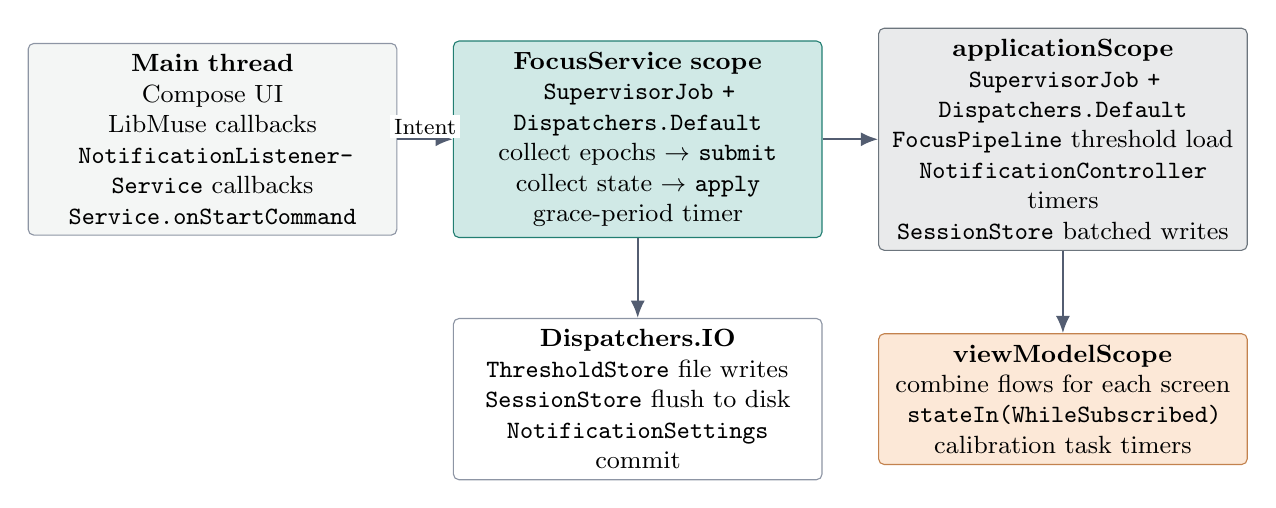
\begin{tikzpicture}[font=\small,every node/.append style={text width=44mm,align=left}]
  \node[box,fill=paper] at (0,0) (main){\textbf{Main thread}\\
    Compose UI\\LibMuse callbacks\\\code{NotificationListener\-Service} callbacks\\
    \code{Service.onStartCommand}};
  \node[wabox] at (5.4,0) (svc){\textbf{FocusService scope}\\
    \code{SupervisorJob + Dispatchers.Default}\\collect epochs $\to$ \code{submit}\\
    collect state $\to$ \code{apply}\\grace-period timer};
  \node[wsbox] at (10.8,0) (app){\textbf{applicationScope}\\
    \code{SupervisorJob + Dispatchers.Default}\\\code{FocusPipeline} threshold load\\
    \code{NotificationController} timers\\\code{SessionStore} batched writes};
  \node[box] at (5.4,-3.3) (io){\textbf{Dispatchers.IO}\\
    \code{ThresholdStore} file writes\\\code{SessionStore} flush to disk\\
    \code{NotificationSettings} commit};
  \node[wdbox] at (10.8,-3.3) (vm){\textbf{viewModelScope}\\
    combine flows for each screen\\\code{stateIn(WhileSubscribed)}\\
    calibration task timers};
  \draw[flow](main.east)--(svc.west) node[midway,above,lbl,text width=,align=center]{Intent};
  \draw[flow](svc)--(app);
  \draw[flow](svc)--(io);
  \draw[flow](app)--(vm);
\end{tikzpicture}}
\caption{Where code runs. Shared mutable state between these is guarded either by a
\code{StateFlow} (the normal case) or by an explicit lock (\code{FocusPipeline.submit/reset},
\code{DeferralQueue}, \code{NotificationController}'s mutex, \code{DndController}).}\label{fig:threads}
\end{figure}

The rule of thumb is that platform callbacks arrive on the main thread, every long-lived loop
lives in a \code{SupervisorJob} scope on \code{Dispatchers.Default}, and the only places that
touch disk hop to \code{Dispatchers.IO}. State crosses between them almost exclusively as
\code{StateFlow}s, which is why nearly every class in the project exposes one.

\subsection{Android platform pieces}

\file{AndroidManifest.xml} was written in sprint~0 so that the four workloads never raced on it.
It declares three components and the permissions in \cref{tab:perms}.

\begin{itemize}
\item \code{FocusApp} as the \code{Application} class.
\item \code{MainActivity}, the single activity hosting the Compose navigation graph. It also
  carries the \code{AUTOMATIC\_ZEN\_RULE} intent filter and the
  \code{ruleType}/\code{ruleInstanceLimit} meta-data, because the Do Not Disturb rule names it as
  its configuration activity.
\item \code{service.FocusService} with \code{foregroundServiceType="connectedDevice"}, not
  exported.
\item \code{notification.FocusNotificationListener}, exported, guarded by the system-only
  \code{BIND\_NOTIFICATION\_\allowbreak LISTENER\_SERVICE} permission, with the
  \code{NotificationListenerService} intent filter.
\end{itemize}

\begin{table}[htbp]\centering\small
\begin{tabularx}{\textwidth}{@{}l l X@{}}
\toprule
\textbf{Permission} & \textbf{Kind} & \textbf{Why} \\
\midrule
\code{BLUETOOTH\_SCAN} (\code{neverForLocation}) & runtime, 31+ & Find the headband. Without the flag,
  Android~12+ silently drops every scan result unless fine location is also held. \\
\code{BLUETOOTH\_CONNECT} & runtime, 31+ & Connect to it. \\
\code{ACCESS\_FINE\_LOCATION} (\code{maxSdk 30}) & runtime & Pre-31 equivalent for BLE scanning. \\
\code{BLUETOOTH}, \code{BLUETOOTH\_ADMIN} (\code{maxSdk 30}) & install & Legacy, still required by some
  LibMuse-internal calls. \\
\code{FOREGROUND\_SERVICE}, \code{FOREGROUND\_SERVICE\_CONNECTED\_DEVICE} & install & Host the BLE link
  and decision loop; Android~14+ requires the typed permission. \\
\code{POST\_NOTIFICATIONS} & runtime, 33+ & The service notification and the catch-up summary. \\
\code{ACCESS\_NOTIFICATION\_POLICY} & special access & Create and toggle the \code{AutomaticZenRule}. \\
\code{REQUEST\_IGNORE\_BATTERY\_OPTIMIZATIONS} & special access & Ask to be exempt from Doze and OEM
  battery killers. \\
Notification listener access & special access & Granted in system Settings, not via a dialog. Lets
  the listener see what arrived while focused. \\
\bottomrule
\end{tabularx}
\caption{Permissions declared in the manifest and requested by D's onboarding flow.}\label{tab:perms}
\end{table}

\begin{gotcha}[The \code{neverForLocation} flag was the first headset bug]
The app originally scanned forever and \code{museListChanged()} never fired, although the phone
could see \code{Muse-3973} advertising. \code{BLUETOOTH\_SCAN} without
\code{usesPermissionFlags="neverForLocation"} only receives results when the app also holds
\code{ACCESS\_FINE\_LOCATION}, which is capped at SDK~30 here and so can never be granted on a modern
phone. LibMuse's \code{startListening()} swallows the exception, so nothing surfaced. The fix is one
attribute in the manifest. The full account is in \file{MUSE\_CONNECTION\_FIXES.md}~\S1.
\end{gotcha}

\paragraph{Build.} \file{app/build.gradle.kts} targets SDK~37 with \code{minSdk = 26}, Kotlin
2.2 with the Compose compiler plugin, and Material~3 through the Compose BOM. LibMuse is a plain
\code{libmuse\_android.jar} in \file{app/libs}, picked up by the \code{fileTree} dependency. The
only non-Compose libraries are Navigation Compose, DataStore Preferences and
\code{kotlinx-coroutines-test}. Each workload owns its own \file{strings\_*.xml} so the resource
files never conflict. Gradle needs \code{JAVA\_HOME} set, and the emulator is not usable on the
development machine, so testing has been on a physical phone over wireless \code{adb}.
% =============================================================================
\section{Workload A: sensing and the foreground service}\label{sec:a}
% =============================================================================

\begin{files}
\file{device/MuseEegSource.kt}, \file{device/ForegroundEegSource.kt}, \file{device/OscEegSource.kt},
\file{device/FakeEegSource.kt}, \file{service/FocusService.kt}, \file{MainActivity.kt},
\file{MUSE\_CONNECTION\_FIXES.md}, \file{docs/area\_specific\_changes.md} (Workload A)
\end{files}

Workload A owns two things: getting a usable \code{FocusEpoch} out of the headset once a second,
and the foreground service that keeps the decision loop alive with no screen open. The first is
mostly a fight with LibMuse's undocumented behaviour; the second is mostly a fight with Android's
power management. Both are documented in the two markdown files above, which are worth reading
in full because they record what was observed on the phone, not just what was changed.

\subsection{\code{MuseEegSource}: the production source}

The class wraps Interaxon's LibMuse SDK (a plain \code{libmuse\_android.jar} in \file{app/libs}
plus native libraries under \file{jniLibs}). It subscribes to LibMuse's pre-computed relative
band powers, the horseshoe contact indicator, accelerometer, battery and artifact packets, and
once per second reduces them to one epoch. It also owns the whole scan, connect, drop and rescan
lifecycle, shown in \cref{fig:muse-lifecycle}.

\begin{figure}[htbp]\centering
\resizebox{\textwidth}{!}{%
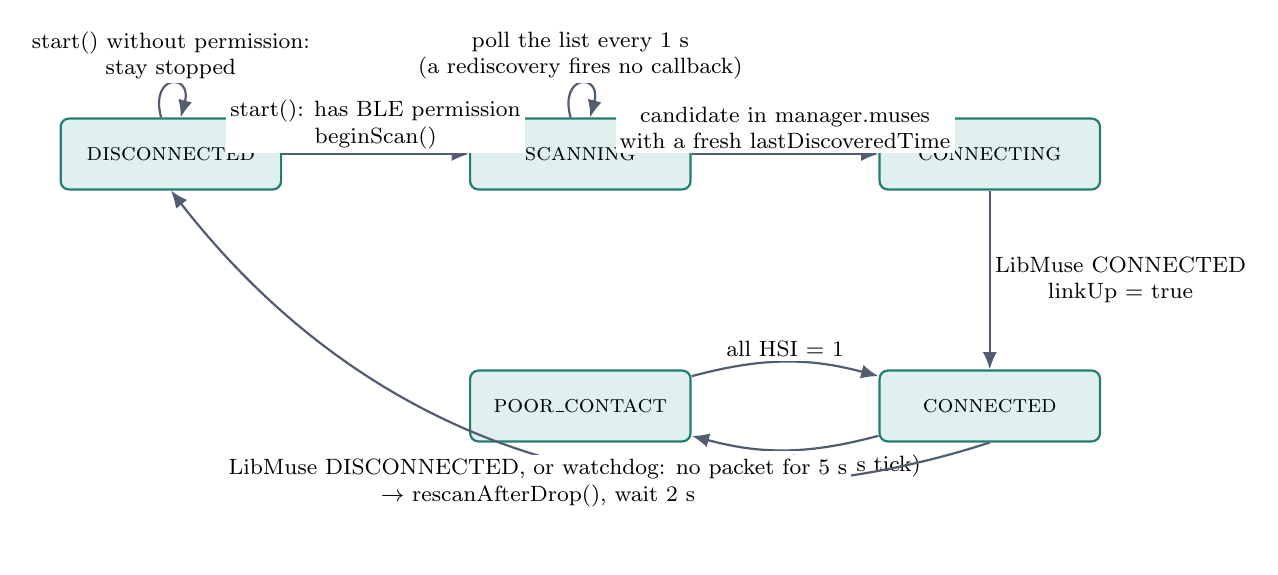
\begin{tikzpicture}[font=\small,
  st/.style={draw=wa!80!black,thick,rounded corners=3pt,fill=wa!15,minimum width=28mm,minimum height=9mm,align=center,font=\small\scshape},
  el/.style={lbl,font=\footnotesize,align=center}]
  \node[st] at (0,0)    (dis){disconnected};
  \node[st] at (5.2,0)  (scan){scanning};
  \node[st] at (10.4,0) (conn){connecting};
  \node[st] at (10.4,-3.2) (ok){connected};
  \node[st] at (5.2,-3.2)  (poor){poor\_contact};
  \draw[flow](dis)--(scan) node[midway,above,el]{start(): has BLE permission\\beginScan()};
  \draw[flow](scan)--(conn) node[midway,above,el]{candidate in manager.muses\\with a fresh lastDiscoveredTime};
  \draw[flow](conn)--(ok) node[midway,right,el]{LibMuse CONNECTED\\linkUp = true};
  \draw[flow](ok) to[bend left=15] node[midway,below,el]{any HSI $>$ 1 (per 1 s tick)} (poor);
  \draw[flow](poor) to[bend left=15] node[midway,above,el]{all HSI = 1} (ok);
  \draw[flow](ok.south) to[bend left=35] node[pos=0.5,below,el]{LibMuse DISCONNECTED, or watchdog: no packet for 5 s\\$\to$ rescanAfterDrop(), wait 2 s} (dis.south);
  \draw[flow](scan) to[loop above,looseness=6] node[above,el]{poll the list every 1 s\\(a rediscovery fires no callback)} (scan);
  \draw[flow](dis) to[loop above,looseness=6] node[above,el]{start() without permission:\\stay stopped} (dis);
\end{tikzpicture}}
\caption{The Muse source's connection lifecycle as the rest of the app sees it through
\code{DeviceStatus.state}. Only \textsc{connected} counts as \code{usable}.}\label{fig:muse-lifecycle}
\end{figure}

\paragraph{Starting} (\file{MuseEegSource.kt:89}). \code{start()} is idempotent via a
\code{stopped} flag. If the Bluetooth runtime permissions are missing it logs, publishes
\textsc{disconnected} and returns \emph{without} clearing \code{stopped}, so the next
\code{start()} after onboarding grants access really scans. The earlier behaviour set the flag with
no scan running, and every later start returned early until the process was killed. Otherwise it
installs the LibMuse listener, calls \code{beginScan()} and launches the tick and watchdog loops.

\paragraph{Finding the headband.} LibMuse only fires \code{museListChanged()} for a headband it has
never seen before. One already in its internal list, which is the normal case after a drop or an
app restart, is silently ``rediscovered'' with a timestamp update and no callback. So
\code{beginScan()} calls \code{connectToAvailableMuse()} directly after \code{startListening()}
and then polls the list every second until something connects. The selection is
\code{@Synchronized} because it is reached both from the main-thread callback and from the
polling coroutine.

\paragraph{Not reconnecting to a ghost.} After a drop LibMuse keeps the headband listed for
about 30\,s with its old discovery time. Connecting to that entry while the headband is switched
off just times out, showing ``Connecting'' the whole while. \code{rescanAfterDrop()} therefore
records the headband\textquotesingle s \code{lastDiscoveredTime} as the stale time, and the
selection in \code{connectToAvailableMuse()} only takes an entry whose time is newer, meaning the
headband is genuinely advertising again.

\paragraph{Connecting} (\file{MuseEegSource.kt:196}). \code{connectTo()} resets the per-connection
band state, registers listeners for exactly eight packet types (the four \code{*\_RELATIVE} bands,
\code{ACCELEROMETER}, \code{HSI\_PRECISION}, \code{BATTERY}, \code{ARTIFACTS}), sets
\code{PRESET\_21} and calls \code{runAsynchronously()}. LibMuse's connection listener then drives
the state: \code{CONNECTED} sets the \code{@Volatile linkUp} flag and stamps
\code{lastPacketAtMs} so the watchdog does not fire before the first packet;
\code{DISCONNECTED} triggers a rescan after 2\,s; \code{NEEDS\_UPDATE} and \code{NEEDS\_LICENSE}
drop to \textsc{disconnected} with no retry.

\paragraph{Drop detection} is belt and braces: LibMuse's own \code{DISCONNECTED} callback, plus a
watchdog that treats 5\,s without any data packet while \textsc{connected} or
\textsc{poor\_contact} as a drop. Both paths go through \code{rescanAfterDrop()}.

\subsubsection{From packets to an epoch}

LibMuse callbacks arrive on the main thread, so the per-tick accumulators are guarded by
\code{synchronized(lock)}. The data listener stores each band packet through \code{mergeFresh()}
(\file{MuseEegSource.kt:273}), which is the single most important hack in the file.

\begin{why}[Why \code{mergeFresh} compares every channel against the previous packet]
For the relative band packets LibMuse sends \code{NaN} for a channel until it has its first clean
window, and afterwards \emph{repeats the last clean value} while it rejects the current window for
a blink or poor contact. Averaging all four channels meant one \code{NaN} channel made the whole
index \code{NaN}, and repeated values were treated as fresh data; in one session the frontal alpha
did not change for three and a half minutes. \code{mergeFresh} keeps only per-channel values that
are finite and differ from the previous packet, and a channel with nothing fresh this tick stays
\code{NaN}. The first focus value then appeared about a second after contact settled, instead of
about ninety.
\end{why}

Every \code{periodMs} (1\,s) \code{emitEpoch()} (\file{MuseEegSource.kt:320}) snapshots and clears
the accumulators, and then:

\begin{enumerate}
\item Returns without emitting if there is no active headband or \code{linkUp} is false. Deriving
  state from an empty horseshoe during a reconnect is what used to show ``Poor contact'' instead of
  ``Connecting''.
\item Publishes \textsc{connected} if every electrode's HSI is 1, otherwise \textsc{poor\_contact}.
\item Reduces the bands: \code{alphaTemporal} is the mean of channels 0 and 3 (TP9 and TP10),
  \code{beta1320}, \code{theta} and \code{emgBroadband} are four-channel means of LibMuse's beta,
  theta and gamma. The averages skip \code{NaN} channels and return \code{NaN}, not 0, when none
  remain, so missing data can never produce a plausible-looking index.
\item Sets \code{ArtifactFlags} from the sticky blink and jaw-clench flags, from an accelerometer
  delta norm above 0.6, and from an EMG rule \code{gamma > 3.0 \&\& beta > 3.0}.
\item Sets \code{valid} to true only if no flag is set, contact is all good and the index is finite,
  then \code{tryEmit}s the epoch on a shared flow with an 8-slot buffer.
\end{enumerate}

\begin{gotcha}[Three things to say honestly if asked]
The field names in \code{BandPowers} promise 13--20\,Hz beta and 20--40\,Hz EMG, but the Muse
source fills them with LibMuse's whole beta band and its gamma band; the clamp is a contract, not
something this source enforces. LibMuse's relative band powers are fractions in $[0,1]$, so the
EMG rule with thresholds of 3.0 can never fire on this source. And on the phone roughly one epoch
in three was invalid for blinks, with AF8 at HSI~2 the next most common cause, because
\code{allGood} demands every electrode at exactly 1.
\end{gotcha}

\subsection{\code{ForegroundEegSource}: keep the headset connected while the app is open}

A 35-line decorator using Kotlin interface delegation (\code{EegSource by inner}) that overrides
only \code{stop()}. \code{hold()} sets a flag and starts the inner source; \code{release(keepConnected)}
clears the flag and stops it unless a session is running; and while held, \code{stop()} is
ignored. \code{MainActivity} calls \code{hold()} from \code{onResume()} and \code{release()} from
\code{onStop()}, skipping the release on configuration changes so rotation does not drop BLE.

\begin{why}[Why \code{onResume} and not \code{onStart}, and why ignore \code{stop()}]
The runtime permission dialog only pauses the activity, and the first real scan has to happen
after the grant, so the hold must be re-run on resume. Calibration and \code{FocusService} both
call \code{stop()} when they finish; honouring it would drop the headset with the app still
visible, and before this wrapper existed the headset only connected once calibration started,
which ate into the 45\,s baseline countdown.
\end{why}

\subsection{The other two sources}

\paragraph{\code{OscEegSource}} is the prototyping shortcut from \file{DESIGN.md}~\S5: the Mind
Monitor app streams Muse data as OSC messages over UDP, and this class listens on port 5000 and
produces the same epochs. The receive loop runs on \code{Dispatchers.IO} because
\code{DatagramSocket.receive()} blocks; shared state is behind a coroutine \code{Mutex} rather than
\code{synchronized} because, unlike LibMuse, all its writers are coroutines. The private
\code{OscDecoder} handles the subset of OSC that Mind Monitor sends: a \code{/}-prefixed address,
a type-tag string, and big-endian \code{f}, \code{i}, \code{T}, \code{F} and \code{s} arguments,
all 4-byte aligned. \Cref{tab:osc} lists the addresses it understands. Two quirks matter if you
swap it in: it publishes \textsc{poor\_contact} one second after start regardless of whether any
packet arrived, and it uses Mind Monitor's \code{\_absolute} bands where the Muse source uses
LibMuse's \code{\_RELATIVE} ones, so the index and the EMG thresholds are on a different scale.

\begin{table}[htbp]\centering\small
\begin{tabular}{@{}l l l@{}}
\toprule
\textbf{OSC address} & \textbf{Arguments} & \textbf{Used for} \\
\midrule
\code{/muse/elements/alpha\_absolute} etc. & 4 floats, TP9 AF7 AF8 TP10 & the four bands \\
\code{/muse/elements/horseshoe} & 4 floats, 1/2/4 & \code{ContactQuality} \\
\code{/muse/elements/blink}, \code{jaw\_clench} & 1 float, $>0$ & sticky artifact flags \\
\code{/muse/acc} & 3 floats & movement if delta norm $>0.6$ \\
\code{/muse/batt} & first arg & battery, divided by 10 \\
\bottomrule
\end{tabular}
\caption{Mind Monitor messages parsed by \code{OscEegSource.handleMessage}.}\label{tab:osc}
\end{table}

\paragraph{\code{FakeEegSource}} is the headset-free source that let B, C and D run the app on
day one. It fakes a connection (\textsc{scanning}, 400\,ms, \textsc{connecting}, 600\,ms,
\textsc{connected} at 87\,\% battery), then emits one epoch per second from a seeded random
generator. ``True focus'' $f$ follows a 180\,s raised-cosine cycle, and the bands are linear in
$f$ with uniform jitter: $\beta = 3 + 4f$, $\alpha = 4 - 2f$, $\theta = 3 - f$, so the index runs
from about 0.43 to 1.75 (\cref{fig:fake}). Five percent of epochs carry one random artifact flag,
and every 97 epochs there is a five-epoch poor-contact episode. It is no longer selectable at
runtime: a settings switch existed for about an hour during integration and was removed, so using
it means editing the one line in \file{AppContainer.kt}. Do not confuse it with D's
\code{DemoEegSource} in \file{ui/preview/DemoStack.kt}, which backs Compose previews.

\begin{figure}[htbp]\centering
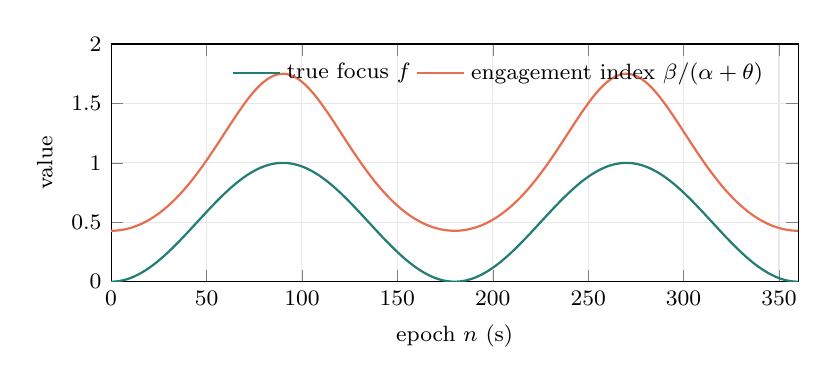
\begin{tikzpicture}
\begin{axis}[width=0.85\textwidth,height=4.6cm,xlabel={epoch $n$ (s)},ylabel={value},
  xmin=0,xmax=360,ymin=0,ymax=2,legend pos=north east,legend style={font=\footnotesize,draw=none,fill=none},
  grid=major,grid style={slate!15},tick label style={font=\footnotesize},label style={font=\footnotesize},
  legend columns=2]
\addplot[wa!80!black,thick,domain=0:360,samples=181]{(sin(deg(2*pi*mod(x,180)/180 - pi/2))+1)/2};
\addlegendentry{true focus $f$}
\addplot[wb,thick,domain=0:360,samples=181]{(3+4*((sin(deg(2*pi*mod(x,180)/180 - pi/2))+1)/2))/(7-3*((sin(deg(2*pi*mod(x,180)/180 - pi/2))+1)/2))};
\addlegendentry{engagement index $\beta/(\alpha+\theta)$}
\end{axis}
\end{tikzpicture}
\caption{What \code{FakeEegSource} generates, before jitter and artifacts. Note the cycle ignores
whatever calibration block is running, which is why a calibration on the fake source is usually
non-separable.}\label{fig:fake}
\end{figure}

\subsection{\code{FocusService}: the decision loop}

The service is declared with \code{foregroundServiceType="connectedDevice"}, is not exported, and
is not bound: \code{onBind} returns null. It is started and stopped with plain intents through the
companion \code{start(context)} and \code{stop(context)}, and the UI observes it through two
companion-object \code{MutableStateFlow}s, \code{isRunning} and \code{appliedState}, which
\code{AndroidServiceController} exposes as the \code{ServiceController} contract. If the process
dies those flows reset to false and \state{unknown}, which is the honest answer to ``did Doze kill
it?''. \code{onStartCommand} returns \code{START\_STICKY} so the system recreates the service after
killing the process, and because all the wiring is in \code{onCreate}, a sticky restart restarts
the loop.

\code{onCreate} resolves the container, creates the \code{focus\_service} channel at
\code{IMPORTANCE\_LOW} (an app for reducing interruptions must not itself interrupt), calls
\code{startForeground} with notification id 1001 and the connected-device type, logs whether the
app is exempt from battery optimisation, and launches \code{runDecisionLoop()}
(\file{FocusService.kt:97}), which does the following in order:

\begin{enumerate}
\item \code{focusEngine.reset()} and \code{sessionRecorder.onSessionStart()}.
\item \code{startWithReconnectBackoff()}: start the source, then watch its status. When it becomes
  usable, reset the backoff to 2\,s; when it drops to \textsc{disconnected} after having been
  usable, wait, call \code{start()} again, and double the wait up to 30\,s. For the Muse source
  this is largely redundant because it rescans by itself, but it matters for a source whose
  \code{start()} really reopens something.
\item Collect \code{epochs} into \code{focusEngine.submit}.
\item Build \code{signalUsable}: the status mapped to \code{usable}, \code{distinctUntilChanged},
  then \code{mapLatest} so that a drop only becomes ``false'' after \code{SIGNAL\_GRACE\_MS}
  (10\,s) and is cancelled if the signal comes back first.
\item Combine that with \code{focusEngine.state} into an effective state: the engine's state when
  usable, otherwise \state{unknown}. On every change: if \state{unknown} and anything is held,
  \code{flush(HEADSET\_REMOVED)} and \code{focusEngine.reset()}; then \code{suppressor.apply()},
  publish \code{appliedState}, and update the service notification text.
\item A second \code{mapLatest} on usability that calls \code{stopSelf()} after
  \code{STOP\_AFTER\_SIGNAL\_LOSS\_MS} (120\,s) without signal. A headset that stays away is a
  session that is over.
\item Collect \code{decisions} into \code{sessionRecorder.onDecision}.
\end{enumerate}

\begin{figure}[htbp]\centering
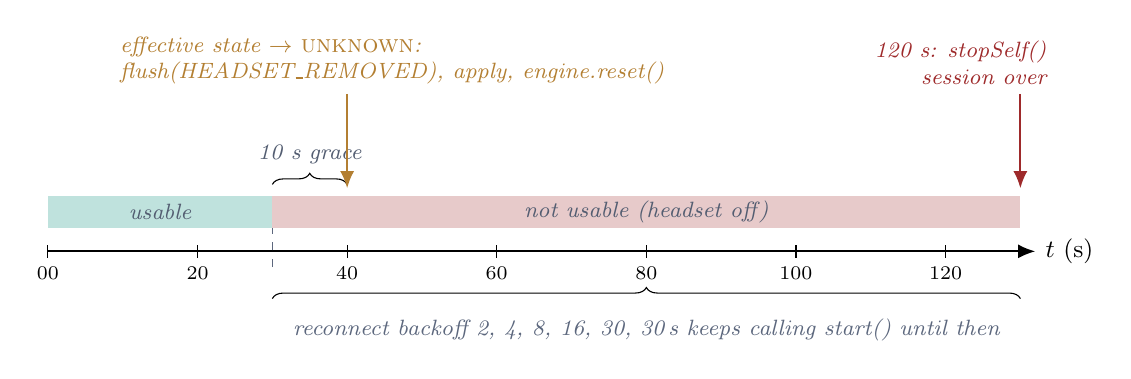
\begin{tikzpicture}[font=\small,x=0.95cm]
  \draw[->,thick](0,0)--(13.2,0) node[right]{$t$ (s)};
  \foreach \x in {0,2,...,12} \draw(\x,0.08)--(\x,-0.08) node[below,font=\scriptsize]{\x0};
  % usable bar
  \fill[wa!30](0,0.3)rectangle(3,0.7); \fill[rust!25](3,0.3)rectangle(13,0.7);
  \node[note] at (1.5,0.5){usable}; \node[note] at (8,0.5){not usable (headset off)};
  % grace
  \draw[decorate,decoration={brace,amplitude=4pt}](3,0.85)--(4,0.85) node[midway,above=4pt,note]{10 s grace};
  \draw[thick,amber!80!black,->](4,2.0)--(4,0.8); \node[above,note,text=amber!80!black,align=left] at (4.6,2.0){effective state $\to$ \state{unknown}:\\flush(HEADSET\_REMOVED), apply, engine.reset()};
  \draw[decorate,decoration={brace,amplitude=4pt}](3,-0.6)--(13,-0.6); % dummy for spacing
  \draw[thick,rust,->](13,2.0)--(13,0.8); \node[above,note,text=rust,align=right] at (12.2,2.0){120 s: stopSelf()\\session over};
  \draw[dashed,slate](3,-0.2)--(3,0.3);
  \node[note,text=slate] at (8,-1.0){reconnect backoff 2, 4, 8, 16, 30, 30\,s keeps calling start() until then};
\end{tikzpicture}
\caption{Signal loss in \code{FocusService}. A blip shorter than the grace period changes nothing;
after it the service fails open, and after two minutes it ends the session.}\label{fig:grace}
\end{figure}

\begin{why}[Why the grace period and the reset on loss]
On the phone a single electrode reading HSI~2 for four seconds used to release the whole queue and
toggle DND off and on. \code{mapLatest} with a 10\,s delay makes a loss count only once it has
lasted. The \code{reset()} on loss means a reconnect has to re-earn \state{focused} through the
entry dwell rather than resuming the instant the link is back. The old
\code{watchForHeadsetRemoved()} was removed because it counted emissions of a \code{StateFlow},
which only emits on change, so it never counted five of anything.
\end{why}

\code{onDestroy} fails open on the way out: cancel the loop job, stop the source (a no-op while
\code{ForegroundEegSource} is held), set the companion flows to false and \state{unknown}, and
then on the scope \code{apply(UNKNOWN)}, \code{flush(SERVICE\_STOPPED)} and
\code{onSessionEnd()}. There are no wake locks anywhere; the service relies on foreground status,
LibMuse's BLE callbacks and the battery-optimisation exemption requested in onboarding.

\begin{why}[Why \code{runDecisionLoop()} is a \code{coroutineScope} block]
Every collector inside it is started with a bare \code{launch}, so each is a child of the loop
coroutine and therefore of \code{loopJob}; \code{startWithReconnectBackoff()} is an extension on
that same scope for the same reason. Cancelling \code{loopJob} in \code{onDestroy} then stops all
of them. An earlier version launched them on the service's own \code{scope} as siblings, so
\code{loopJob?.cancel()} cancelled a coroutine that had already returned and the collectors
outlived the service: with the app in the foreground the headset stayed connected, epochs kept
feeding the app-wide engine, and the leaked state collector kept calling \code{apply()} and
overwriting \code{appliedState} after \code{onDestroy} had set it to \state{unknown}. The service's
\code{scope} is still used for two things only: launching \code{loopJob}, and the fail-open work in
\code{onDestroy} that must outlive the cancelled loop.
\end{why}
% =============================================================================
\section{Workload B: signal processing and calibration}\label{sec:b}
% =============================================================================

\begin{files}
\file{signal/FocusPipeline.kt}, \file{signal/ArtifactRejector.kt}, \file{signal/FocusStateMachine.kt},
\file{signal/DriftDetector.kt}, \file{calibration/CalibrationSession.kt},
\file{calibration/ThresholdFitter.kt}, \file{data/ThresholdStore.kt}, \file{SUMMARY\_B.md} (partly stale,
see \cref{sec:integration}), tests under \file{test/.../signal/}, \file{calibration/} and
\file{data/ThresholdStoreTest.kt}
\end{files}

This is the research contribution and the part of the codebase with the most numbers in it. It is
almost all pure Kotlin with no Android dependency, which is why it carries about a hundred unit
tests and why it is the easiest workload to reason about from the tests alone. Everything in this
section is reachable from one method, \code{FocusPipeline.decide()}, so that is where to start
reading.

\subsection{The pipeline per epoch}\label{sec:b:pipeline}

\begin{figure}[htbp]\centering
\resizebox{\textwidth}{!}{%
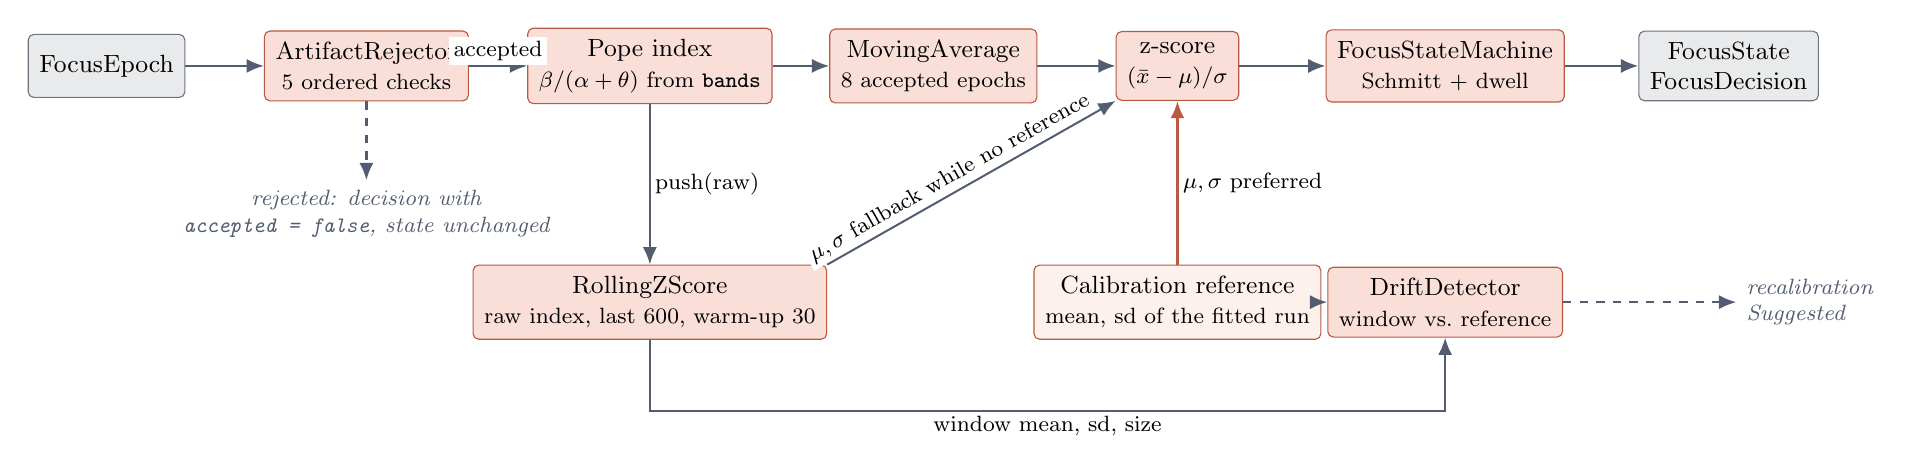
\begin{tikzpicture}[font=\small]
  \node[wsbox] at (0,0)    (ep){FocusEpoch};
  \node[wbbox] at (3.3,0)  (rej){ArtifactRejector\\\footnotesize 5 ordered checks};
  \node[wbbox] at (6.9,0)  (idx){Pope index\\\footnotesize $\beta/(\alpha+\theta)$ from \code{bands}};
  \node[wbbox] at (10.5,0) (ma){MovingAverage\\\footnotesize 8 accepted epochs};
  \node[wbbox] at (13.6,0) (z){z-score\\\footnotesize $(\bar x - \mu)/\sigma$};
  \node[wbbox] at (17.0,0) (sm){FocusStateMachine\\\footnotesize Schmitt + dwell};
  \node[wsbox] at (20.6,0) (out){FocusState\\FocusDecision};
  \node[wbbox] at (6.9,-3.0)  (win){RollingZScore\\\footnotesize raw index, last 600, warm-up 30};
  \node[wbbox,fill=wb!10] at (13.6,-3.0) (ref){Calibration reference\\\footnotesize mean, sd of the fitted run};
  \node[wbbox] at (17.0,-3.0) (dr){DriftDetector\\\footnotesize window vs.\ reference};
  \draw[flow](ep)--(rej);
  \draw[flow](rej)--(idx) node[midway,above,lbl]{accepted};
  \draw[flow](idx)--(ma);
  \draw[flow](ma)--(z);
  \draw[flow](z)--(sm);
  \draw[flow](sm)--(out);
  \draw[flow](idx.south)--(win.north) node[midway,right,lbl]{push(raw)};
  \draw[flow](win.north east)--(z.south west) node[pos=0.45,above,sloped,lbl]{$\mu,\sigma$ fallback while no reference};
  \draw[flow,wb!80!black,very thick](ref.north)--(z.south) node[midway,right,lbl]{$\mu,\sigma$ preferred};
  \draw[flow](win.south)--++(0,-0.9)-|(dr.south) node[pos=0.25,below,lbl]{window mean, sd, size};
  \draw[flow](ref.east)--(dr.west);
  \draw[flow,dashed](rej.south)--++(0,-1.0) node[below,note]{rejected: decision with\\\code{accepted = false}, state unchanged};
  \draw[flow,dashed](dr.east)--++(2.2,0) node[right,note,align=left]{recalibration\\Suggested};
\end{tikzpicture}}
\caption{\code{FocusPipeline.decide()}. The smoothed index is scored against the calibration run's
distribution when one exists; the rolling window of \emph{raw} values runs underneath for drift
detection and as the fallback.}\label{fig:pipeline}
\end{figure}

\code{submit(epoch)} (\file{FocusPipeline.kt:109}) takes a lock, runs \code{decide()}, and
\code{tryEmit}s the resulting \code{FocusDecision} on a 128-slot shared flow. \code{decide()}
does, in order:

\begin{enumerate}
\item Recompute the index from \code{epoch.bands.engagementIndex}, never trusting
  \code{epoch.focusIndex}, so the definition lives in one place whichever source made the epoch.
\item Ask the rejector. A rejected epoch yields a decision with \code{accepted = false},
  \code{normalizedZ = 0} and the current state, and touches nothing else.
\item \code{smoother.push(index)}: the mean of the last 8 accepted raw indices (the mean of what is
  there until the window fills; no warm-up).
\item Pick the reference: the calibration run's mean and SD if \code{useCalibrationReference} is on,
  a reference exists, and its SD exceeds $10^{-9}$.
\item \code{rollingZ = normalizer.score(smoothed)}, then \code{normalizer.push(index)}. The window
  holds the \emph{raw} index and scores before adding.
\item $z = (\text{smoothed} - \mu_{\text{ref}})/\sigma_{\text{ref}}$ if there is a reference,
  otherwise \code{rollingZ}, which is null during the 30-epoch warm-up.
\item If $z$ is null or there are no thresholds, return \code{accepted = false}. The smoother and
  window were still fed, so an uncalibrated pipeline is warm the moment thresholds arrive.
\item \code{\_state.value = stateMachine.update(z, timestamp, thresholds)}.
\item \code{drift.check(window mean, sd, size, thresholds.fittedAtMs)}; if true, latch
  \code{recalibrationSuggested}.
\item Return the accepted decision carrying the raw index and $z$.
\end{enumerate}

\begin{why}[Why score against the calibration run and not the rolling window]
This is open question 1 in \file{SUMMARY\_B.md} and the most important change made at
integration. A 10-minute rolling window re-centres on whatever the user has been doing, so during
a long focus period the z-score drifts back to zero and the user drops out of \state{focused}
while still concentrating. The thresholds were fitted against the calibration run's distribution,
so that is what live samples are now scored against. Replaying 620 epochs from a real reading
session with the owner's fitted thresholds gave 0\,\% of the time \state{focused} with the rolling
window and no smoothing, 87\,\% with the calibration reference, and 98\,\% with the reference plus
8-epoch smoothing. The rolling window still runs on raw values underneath so the drift detector
sees exactly what it did before.
\end{why}

\begin{why}[Why smooth, and why keep the window raw]
At 1\,Hz the raw index is noisy enough that a single dip into the dead band resets the entry run,
so ``sustained above $\Thigh$ for 10\,s'' was unreachable: the longest unbroken run in an
11-minute real session was 8\,s. Averaging 8 accepted epochs fixes that and stays well inside the
dwells. The window is fed the raw value because smoothing shrinks the SD, which would look like
spread drift against the calibration reference. The reported \code{normalizedZ} is the smoothed
one so the home chart matches the thresholds drawn on it.
\end{why}

\paragraph{\code{RollingZScore}} (\file{FocusPipeline.kt:240}) keeps the last 600 values (about
10 minutes) and refuses to score until it has 30. It uses the sample SD ($n-1$), returns 0 for a
flat window instead of dividing by zero, and scores a value \emph{before} adding it so a sudden
excursion is not partly cancelled by its own contribution. It is a separate class so the fitter
can normalise exactly the same way.

\paragraph{The other methods.} \code{updateThresholds} saves to the store \emph{before} applying,
so an invalid set is refused by the store's validation rather than half-applied; it leaves the
drift reference alone, so editing a dwell time keeps drift detection working. \code{reset()}
clears the rejector, state machine, window, smoother and the drift counter and sets the state to
\state{unknown}, but keeps the thresholds and does not clear \code{recalibrationSuggested},
because the stale thresholds are still the ones in use next session. The startup load uses
\code{compareAndSet(null, loaded)} so a calibration that lands before the asynchronous disk read
finishes is not overwritten, and restores the drift reference from the history record whose
\code{fittedAtMs} matches the current thresholds.

\subsection{Artifact rejection}

\code{ArtifactRejector.check(epoch)} (\file{ArtifactRejector.kt:57}) returns null to accept or a
\code{RejectReason}. The checks run in the order of \cref{fig:rejector}, and the first hit wins.

\begin{figure}[htbp]\centering
\resizebox{\textwidth}{!}{%
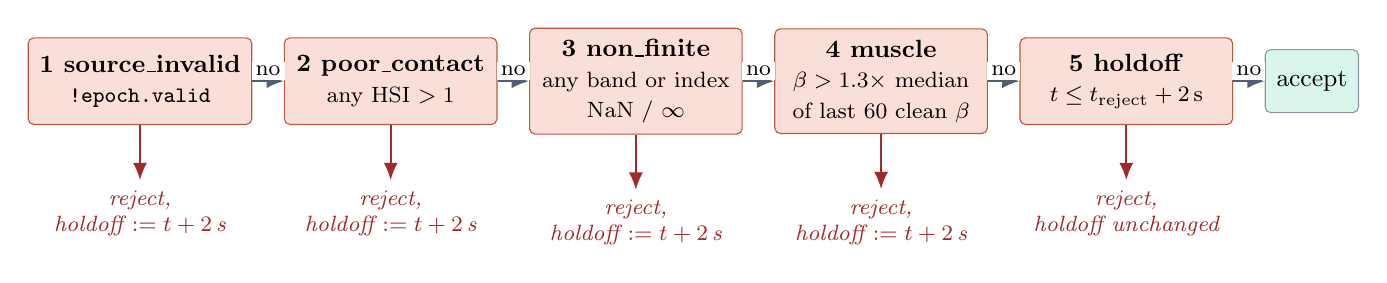
\begin{tikzpicture}[font=\small,node distance=4mm,
  chk/.style={wbbox,minimum width=27mm,minimum height=11mm}]
  \node[chk](c1){\textbf{1 source\_invalid}\\\footnotesize \code{!epoch.valid}};
  \node[chk,right=of c1](c2){\textbf{2 poor\_contact}\\\footnotesize any HSI $>1$};
  \node[chk,right=of c2](c3){\textbf{3 non\_finite}\\\footnotesize any band or index\\\footnotesize NaN / $\infty$};
  \node[chk,right=of c3](c4){\textbf{4 muscle}\\\footnotesize $\beta > 1.3\times$ median\\\footnotesize of last 60 clean $\beta$};
  \node[chk,right=of c4](c5){\textbf{5 holdoff}\\\footnotesize $t \le t_{\text{reject}} + 2\,\text{s}$};
  \node[box,fill=mint!30,right=of c5](ok){accept};
  \foreach \a/\b in {c1/c2,c2/c3,c3/c4,c4/c5,c5/ok} \draw[flow](\a)--(\b) node[midway,above,lbl]{no};
  \foreach \n in {c1,c2,c3,c4} \draw[flow,rust](\n.south)--++(0,-0.7) node[below,note,text=rust]{reject,\\holdoff $:= t+2$\,s};
  \draw[flow,rust](c5.south)--++(0,-0.7) node[below,note,text=rust]{reject,\\holdoff unchanged};
\end{tikzpicture}}
\caption{The rejector's ordered checks. A primary rejection (1--4) restarts the 2\,s holdoff; a
holdoff rejection does not extend it, or one blink would shut the gate forever.}\label{fig:rejector}
\end{figure}

Details that come up in questions:
\begin{itemize}
\item The holdoff is inclusive of its end point: an artifact at $t$ also rejects $t+1$ and $t+2$,
  and $t+3$ is accepted. It exists because artifacts smear across overlapping analysis windows.
\item The muscle rule is relative to the user's own recent beta because absolute band power varies
  between people and sessions. It is skipped until 10 clean epochs exist, and the median is taken
  \emph{before} adding the current epoch.
\item Muscle-rejected epochs still enter the median window. Excluding them would lock the gate
  permanently if baseline beta genuinely rose; with a one-minute window a brief clench cannot move
  the median, while a lasting shift is absorbed within about 60 epochs.
\item \code{reset()} clears both the median window and the holdoff.
\end{itemize}

\begin{gotcha}[The muscle rule may reject real focus]
If concentrating genuinely raises 13--20\,Hz beta by more than 30\,\% over the recent median, the
start of every focus period is thrown away as muscle. A model on the fake source's signal rejected
24\,\% of epochs as muscle and 42\,\% overall. This is open question 2 in \file{SUMMARY\_B.md} and
is unchanged. Note also that A's sources set their own \code{valid} flag with their own EMG rule,
so two layers of artifact logic overlap (open question 3).
\end{gotcha}

\subsection{The Schmitt trigger}

\code{FocusStateMachine.update()} (\file{FocusStateMachine.kt:44}) takes a z-score, its timestamp
and the current thresholds, and is the two-threshold state machine from \file{DESIGN.md}~\S1. It is
fed only accepted z-scores, and
the thresholds are passed in on every call so a changed dwell applies to the run already in
progress.

\begin{figure}[htbp]\centering
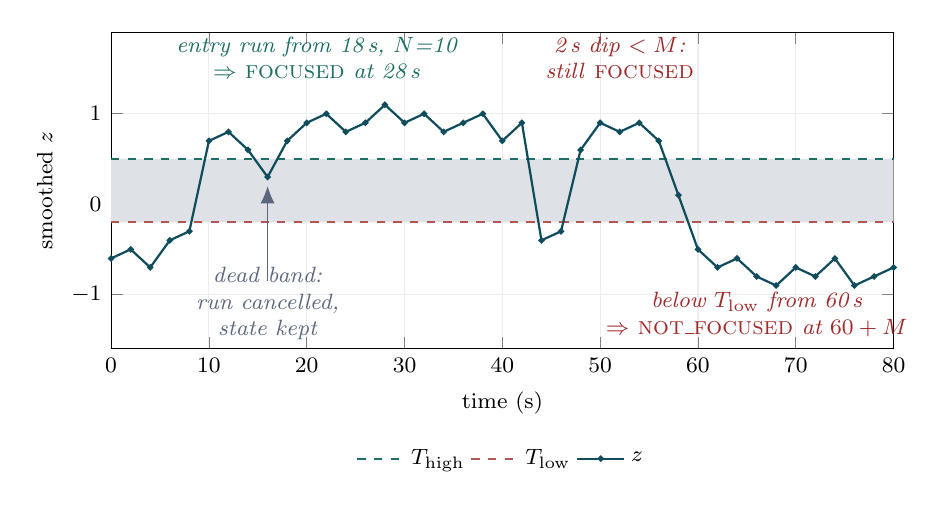
\begin{tikzpicture}
\begin{axis}[width=0.95\textwidth,height=5.6cm,xmin=0,xmax=80,ymin=-1.6,ymax=1.9,clip=false,
  xlabel={time (s)},ylabel={smoothed $z$},grid=major,grid style={slate!12},
  tick label style={font=\footnotesize},label style={font=\footnotesize},
  legend style={font=\footnotesize,draw=none,fill=none,at={(0.5,-0.28)},anchor=north},legend columns=3]
\addplot[name path=th,wa!70!black,dashed,thick,domain=0:80]{0.5}; \addlegendentry{$\Thigh$}
\addplot[name path=tl,rust!80,dashed,thick,domain=0:80]{-0.2}; \addlegendentry{$\Tlow$}
\addplot[slate!20,forget plot] fill between[of=th and tl];
\addplot[teal,thick,mark=*,mark size=0.7pt] coordinates {
 (0,-0.6)(2,-0.5)(4,-0.7)(6,-0.4)(8,-0.3)(10,0.7)(12,0.8)(14,0.6)(16,0.3)(18,0.7)(20,0.9)(22,1.0)
 (24,0.8)(26,0.9)(28,1.1)(30,0.9)(32,1.0)(34,0.8)(36,0.9)(38,1.0)(40,0.7)(42,0.9)(44,-0.4)(46,-0.3)
 (48,0.6)(50,0.9)(52,0.8)(54,0.9)(56,0.7)(58,0.1)(60,-0.5)(62,-0.7)(64,-0.6)(66,-0.8)(68,-0.9)
 (70,-0.7)(72,-0.8)(74,-0.6)(76,-0.9)(78,-0.8)(80,-0.7)};
\addlegendentry{$z$}
\node[note,text=slate] at (axis cs:16,-1.1){dead band:\\run cancelled,\\state kept};
\draw[->,slate] (axis cs:16,-0.85)--(axis cs:16,0.2);
\node[note,text=wa!70!black] at (axis cs:21,1.62){entry run from 18\,s, $N$=10\\$\Rightarrow$ \state{focused} at 28\,s};
\node[note,text=rust] at (axis cs:52,1.62){2\,s dip $< M$:\\still \state{focused}};
\node[note,text=rust] at (axis cs:66,-1.22){below $\Tlow$ from 60\,s\\$\Rightarrow$ \state{not\_focused} at $60+M$};
\end{axis}
\end{tikzpicture}
\caption{The Schmitt trigger with dwell. Defaults before calibration are $\Thigh=+0.5$,
$\Tlow=-0.2$, $N=10$\,s, $M=60$\,s; a fitted set replaces the thresholds, the dwells stay user
settings.}\label{fig:schmitt}
\end{figure}

The algorithm per call:
\begin{enumerate}
\item If more than \code{maxGapMs} (5\,s) has passed since the last sample, discard both runs: a
  gap means the signal was lost, and nothing is known about it.
\item Classify: $z > \Thigh$ starts or continues the high run and clears the low run; $z < \Tlow$
  does the opposite; anything in between (the thresholds themselves included, since comparisons
  are strict) clears both runs but leaves the state alone.
\item Transition: not \state{focused} and the high run has lasted at least \code{entryDwellSec}
  $\Rightarrow$ \state{focused}; not \state{not\_focused} and the low run has lasted at least
  \code{exitDwellSec} $\Rightarrow$ \state{not\_focused}; still \state{unknown} $\Rightarrow$
  \state{not\_focused} (first usable signal fails open); otherwise unchanged.
\end{enumerate}

``Lasted'' is measured between timestamps, \code{now - runStart >= dwell}, not by counting
samples, so at 1\,Hz a 5\,s dwell is satisfied on the sixth sample. The tests pin the consequences:
120 dead-band values hold \state{focused}; alternating 0.4 and 0.6 around $\Thigh = 0.5$ never
chatters because 0.4 is in the dead band, not below $\Tlow$; an 8-second dip below $\Tlow$ with a
10\,s exit dwell does not end focus.

\subsection{Drift detection}

\code{DriftDetector.check(windowMean, windowSd, windowSize, fittedAtMs)}
(\file{DriftDetector.kt:55}) compares the rolling window of raw indices with the calibration
run's mean and SD. It refuses to judge unless a reference exists, its \code{fittedAtMs} matches the
thresholds in use (so the developer placeholder is never judged), and the window holds at least
300 samples (about 5 minutes, half the window). Drift means the mean has moved more than one
reference SD, or the SD ratio is above 2 or below $\tfrac12$; the spread matters because the
thresholds are z-scores, and a changed spread makes the same $z$ a different raw separation. The
condition must hold for 120 consecutive checks, about two minutes, and a single clean check restarts
the count. The detector only says ``now''; the pipeline latches
\code{recalibrationSuggested} until a separable calibration clears it. The reference itself is not
persisted, only rebuilt from the history file at startup, so after a restart it takes roughly
seven minutes of drifted signal before the prompt returns.

\subsection{Calibration: from task blocks to thresholds}

D's calibration screen runs the protocol (nine blocks of 60\,s, three per condition, order
randomised, with a 45\,s baseline and 8\,s rests; \cref{sec:d:calibration}) and collects every
epoch. When it is done it calls \code{FocusEngine.fitCalibration(blocks, epochs)}, and B takes
over (\cref{fig:calib}).

\begin{figure}[htbp]\centering
\resizebox{\textwidth}{!}{%
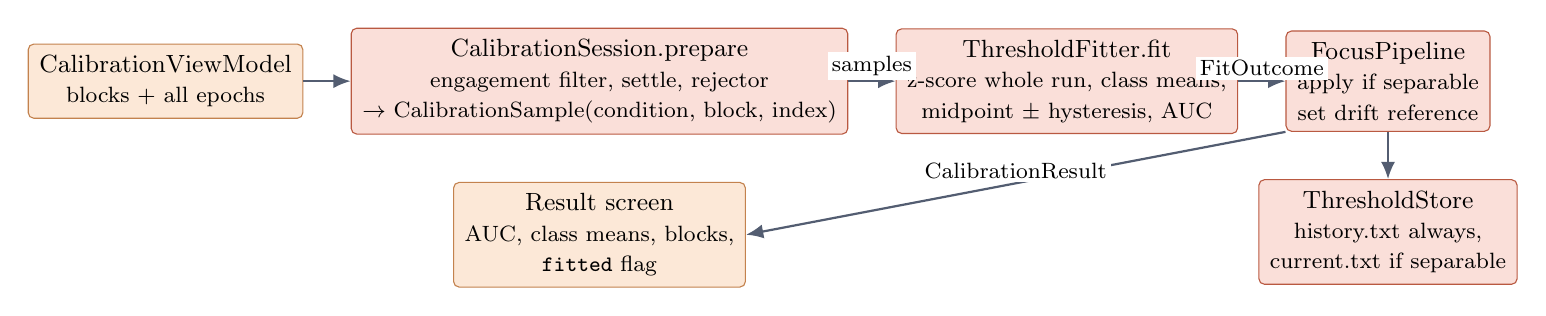
\begin{tikzpicture}[font=\small,node distance=6mm]
  \node[wdbox](vm){CalibrationViewModel\\\footnotesize blocks + all epochs};
  \node[wbbox,right=of vm](ses){CalibrationSession.prepare\\\footnotesize engagement filter, settle, rejector\\\footnotesize $\to$ CalibrationSample(condition, block, index)};
  \node[wbbox,right=of ses](fit){ThresholdFitter.fit\\\footnotesize z-score whole run, class means,\\\footnotesize midpoint $\pm$ hysteresis, AUC};
  \node[wbbox,right=of fit](dec){FocusPipeline\\\footnotesize apply if separable\\\footnotesize set drift reference};
  \node[wbbox,below=of dec](store){ThresholdStore\\\footnotesize history.txt always,\\\footnotesize current.txt if separable};
  \node[wdbox,below=of ses](res){Result screen\\\footnotesize AUC, class means, blocks,\\\footnotesize \code{fitted} flag};
  \draw[flow](vm)--(ses); \draw[flow](ses)--(fit) node[midway,above,lbl]{samples};
  \draw[flow](fit)--(dec) node[midway,above,lbl]{FitOutcome};
  \draw[flow](dec)--(store); \draw[flow](dec.south west)--(res.east) node[midway,above,lbl]{CalibrationResult};
\end{tikzpicture}}
\caption{The calibration path. B labels and fits; D runs the tasks and shows the result.}\label{fig:calib}
\end{figure}

\paragraph{\code{CalibrationSession.prepare}} (\file{CalibrationSession.kt:63}) turns blocks and
epochs into labelled samples:
\begin{itemize}
\item \textbf{Engagement.} \code{MEDIUM} and \code{HIGH} blocks are dropped with a
  \code{DropReason} when the task score is missing (\code{NO\_TASK\_SCORE}), has zero attempts
  (\code{NO\_ATTEMPTS}) or accuracy is below 0.5 (\code{LOW\_ACCURACY}; exactly 0.5 is kept).
  \code{LOW} blocks have no task and are never dropped. A \code{HIGH} block where the user
  disengaged is low-demand data labelled high-demand, the worst input the fitter can get, and
  random pressing on the 2-back scores about 50\,\%.
\item \textbf{Settling.} The first $\min(5\,\text{s}, \text{duration}/12)$ of each block is
  discarded: a 4\,s analysis window plus a second of orienting still contains pre-block signal.
  The fraction keeps the developer's 6\,s fast-mode blocks usable (0.5\,s settle).
\item \textbf{Artifacts.} All epochs, sorted by time, go through one fresh \code{ArtifactRejector},
  so holdoff and the muscle median carry across block boundaries and the fit uses exactly what the
  live pipeline would have accepted.
\item Samples are matched to blocks by wall-clock timestamp (both sides must use the same
  clock), inclusive at both ends, and tagged with the block's
  \emph{position} 0--8 rather than its condition so a future leave-one-block-out evaluation can hold
  out a whole block.
\end{itemize}

\paragraph{\code{ThresholdFitter.fit}} (\file{ThresholdFitter.kt:80}) is pure and stateless:
\begin{enumerate}
\item Drop non-finite indices. If fewer than 10 \code{LOW} or 10 \code{HIGH} samples remain,
  return \code{Insufficient}: that is a failed run, not a calibration.
\item z-score every sample, \code{MEDIUM} included, against the mean and sample SD of the whole run.
  The nine-minute run is about the length of the live window, so these z-scores sit on the same
  scale as live ones; \code{MEDIUM} widens the reference distribution without touching the class
  means or the AUC.
\item Class means $\bar z_{\text{low}}$, $\bar z_{\text{high}}$; midpoint
  $m = (\bar z_{\text{low}} + \bar z_{\text{high}})/2$.
\item Half gap $h = \max\bigl(0.15\,(\bar z_{\text{high}} - \bar z_{\text{low}}),\ 0.05\bigr)$;
  $\Thigh = m + h$, $\Tlow = m - h$. The dead band is 30\,\% of the class separation and never
  narrower than $0.1\,z$, so $\Tlow < \Thigh$ holds even for overlapping or reversed classes.
\item AUC by Mann--Whitney: the fraction of (high, low) pairs where the high sample scores higher,
  ties counting half. It is threshold-free, so it measures the index itself rather than this
  fitting rule, and 0.5 is chance.
\item \code{separable = highMean > lowMean \&\& auc >= 0.6}. Dwell seconds pass through unchanged;
  they are user settings, not fitted.
\end{enumerate}

\begin{figure}[htbp]\centering
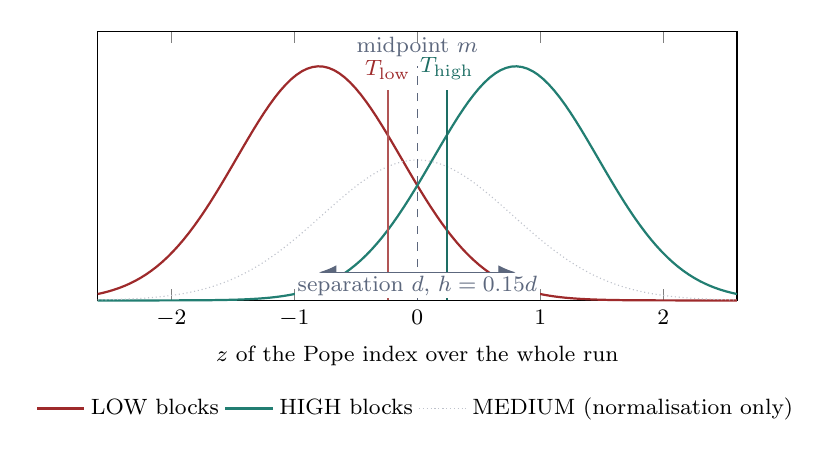
\begin{tikzpicture}
\begin{axis}[width=0.8\textwidth,height=5cm,xmin=-2.6,xmax=2.6,ymin=0,ymax=1.15,clip=false,
  xlabel={$z$ of the Pope index over the whole run},ytick=\empty,
  tick label style={font=\footnotesize},label style={font=\footnotesize},
  legend style={font=\footnotesize,draw=none,fill=none,at={(0.5,-0.32)},anchor=north},legend columns=3]
\addplot[rust,thick,domain=-2.6:2.6,samples=120]{exp(-((x+0.8)^2)/(2*0.45))}; \addlegendentry{LOW blocks}
\addplot[wa!80!black,thick,domain=-2.6:2.6,samples=120]{exp(-((x-0.8)^2)/(2*0.45))}; \addlegendentry{HIGH blocks}
\addplot[slate!40,densely dotted,domain=-2.6:2.6,samples=120]{0.6*exp(-((x)^2)/(2*0.6))}; \addlegendentry{MEDIUM (normalisation only)}
\draw[slate,dashed](axis cs:0,0)--(axis cs:0,1.0) node[above,font=\footnotesize]{midpoint $m$};
\draw[rust!80,thick](axis cs:-0.24,0)--(axis cs:-0.24,0.9) node[above,font=\footnotesize,text=rust]{$\Tlow$};
\draw[wa!70!black,thick](axis cs:0.24,0)--(axis cs:0.24,0.9) node[above,font=\footnotesize,text=wa!70!black]{$\Thigh$};
\draw[<->,slate](axis cs:-0.8,0.12)--(axis cs:0.8,0.12) node[pos=0.5,below,font=\footnotesize,fill=white,inner sep=1pt]{separation $d$, $h=0.15d$};
\end{axis}
\end{tikzpicture}
\caption{What the fitter computes: thresholds sit $\pm15\,\%$ of the class separation either side
of the midpoint between the \code{LOW} and \code{HIGH} means. AUC is the probability a random
\code{HIGH} epoch outscores a random \code{LOW} one.}\label{fig:fitter}
\end{figure}

\paragraph{What the pipeline does with the outcome} (\file{FocusPipeline.kt:161}).
\code{Insufficient} returns a \code{CalibrationResult} with the thresholds already in use, AUC
0.5 and \code{fitted = false}; nothing is saved, and the result screen says ``not enough clean
data'' rather than showing an AUC that was never measured. \code{Fitted} is \emph{always} appended
to the history (poor separability is a finding to report, \file{DESIGN.md}~\S7), but only made
current, applied, and installed as the drift reference if separable. Acting on an index that does
not track this user's engagement would suppress notifications at random, so a non-separable fit
fails open. The result always carries every input block, dropped ones included, so the task
accuracy shown is honest.

\subsection{Persistence: \code{ThresholdStore}}

Two plain-text files under \code{filesDir/thresholds/}: \code{current.txt} holds the thresholds
in use, \code{history.txt} gains one line per calibration and is never rewritten. Each line is
\code{key=value} pairs joined by semicolons, for example:

\begin{center}\small\ttfamily
tHighZ=0.734;tLowZ=-0.12;entryDwellSec=8;exitDwellSec=45;fittedAtMs=1759000000000;auc=0.81;\\
calAuc=0.81;lowMeanZ=-0.6;highMeanZ=0.9;blockCount=9;indexMean=0.42;indexSd=0.07
\end{center}

Everything stored is a z-score, a ratio or a count, never a raw band power. \code{current.txt}
is written to a temp file and renamed into place, because the user can change the exit timeout at
any time and an interrupted write must not leave half a file. \code{validate} refuses non-finite
thresholds, $\Tlow > \Thigh$ and negative dwells. A corrupt history line is skipped; a corrupt
current file reads as ``not calibrated''. Unknown keys are ignored so fields can be added later.
All methods take a \code{Mutex} and run on \code{Dispatchers.IO}.

\begin{why}[Why not JSON or DataStore]
\code{org.json} is a stub on the local JVM, so a JSON store would need Robolectric to test. The
key-value format keeps the twelve store tests plain JUnit, and the pipeline tests can use a real
store in a temporary directory.
\end{why}

\subsection{Constants to have at hand}

\Cref{tab:bconst} collects the numbers that most often come up when this workload is questioned.

\begin{table}[!htbp]\centering\small
\begin{tabularx}{\textwidth}{@{}X l l@{}}
\toprule
\textbf{Constant} & \textbf{Value} & \textbf{Where} \\
\midrule
Smoothing window (production) & 8 epochs & \file{AppContainer.kt} \\
Rolling window / warm-up & 600 / 30 values & \code{RollingZScore} \\
Muscle ratio / median window / min samples & $1.3\times$ / 60 / 10 & \code{ArtifactRejector} \\
Holdoff after a rejection & 2\,s, inclusive & \code{ArtifactRejector} \\
State machine max gap & 5\,s & \code{FocusStateMachine} \\
Placeholder thresholds & $+0.5$, $-0.2$, 10\,s, 60\,s & \code{FocusThresholds.PLACEHOLDER} \\
Drift: mean shift / SD ratio & $>1$ ref SD / $>2$ or $<\tfrac12$ & \code{DriftDetector} \\
Drift: min samples / sustain & 300 / 120 checks & \code{DriftDetector} \\
Settle / fraction / min accuracy & 5\,s / $1/12$ / 0.5 & \code{CalibrationSession} \\
Hysteresis / floor / min per class / min AUC & 0.15 / 0.05\,z / 10 / 0.6 & \code{ThresholdFitter} \\
Real fit on the phone & $\Thigh = +0.23$, $\Tlow = +0.07$, AUC 0.67 & \file{area\_specific\_changes.md} \\
\bottomrule
\end{tabularx}
\caption{Numbers that appear in questions about workload B.}\label{tab:bconst}
\end{table}
% =============================================================================
\section{Workload C: notifications}\label{sec:c}
% =============================================================================

\begin{files}
\file{notification/NotificationController.kt}, \file{notification/DndController.kt},
\file{notification/BreakthroughPolicy.kt}, \file{notification/FocusNotificationListener.kt},
\file{notification/DeferralQueue.kt}, \file{notification/CatchUpNotifier.kt},
\file{data/NotificationSettings.kt}, test \file{notification/NotificationControllerTest.kt},
\file{DESIGN.md}~\S3
\end{files}

The notification layer has the simplest input in the project, a \code{FocusState} once a second,
but the most easily misdescribed behaviour, because most of what happens is done by Android on
the app's behalf. The sentence to get right first: \emph{the app never cancels, snoozes or
re-posts anyone's notifications}. It switches a Do Not Disturb rule on and off, watches what
arrives while the rule is on, and afterwards posts one summary of its own. \file{DESIGN.md}~\S3
calls this ``v1''; snooze-based true deferral is the unbuilt v2 stretch goal.

\subsection{The moving parts}

\begin{figure}[htbp]\centering
\resizebox{\textwidth}{!}{%
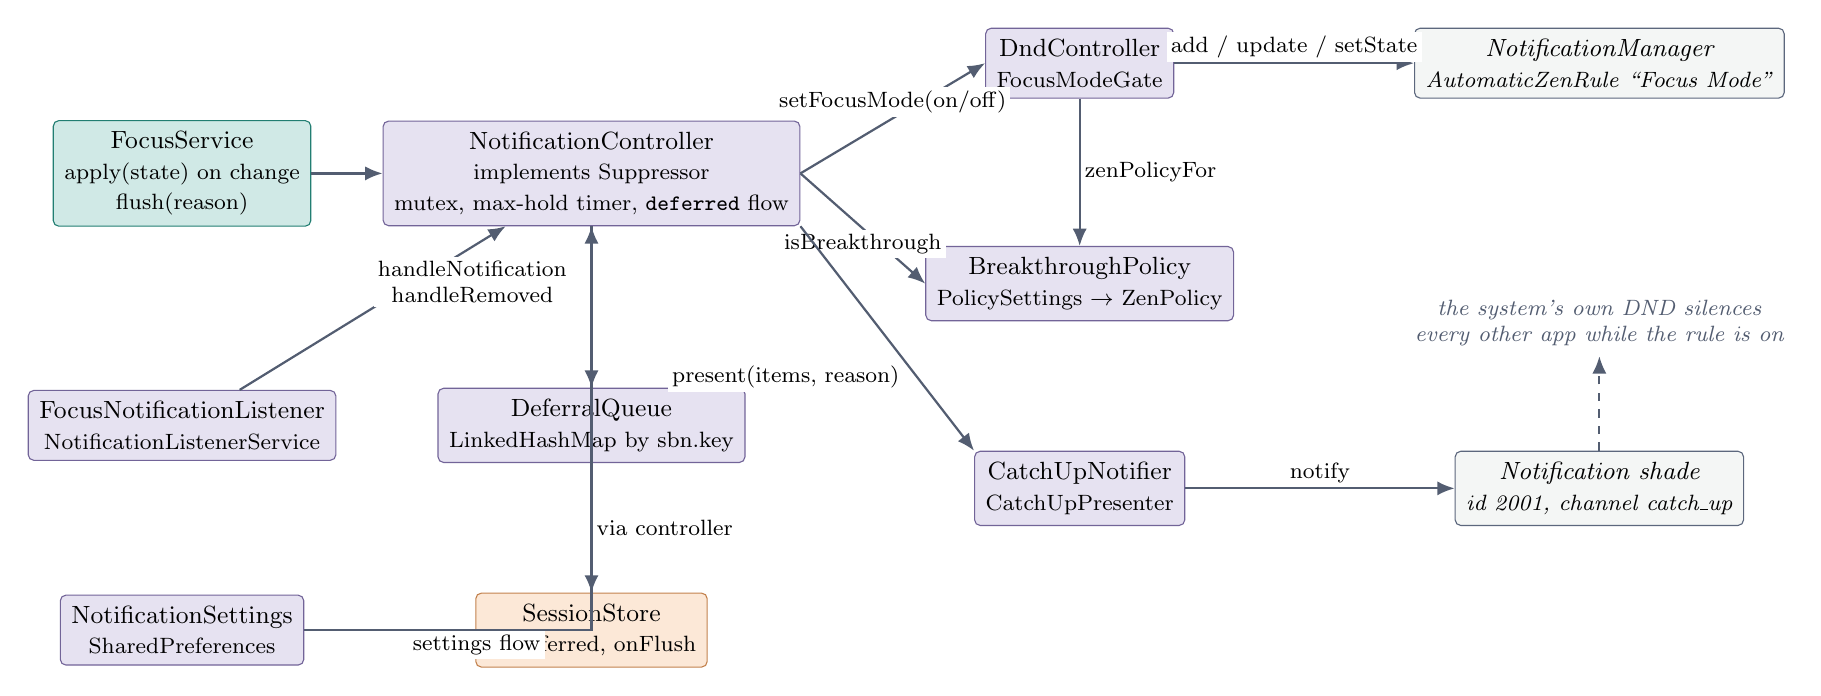
\begin{tikzpicture}[font=\small]
  \node[wabox] at (0,0) (svc){FocusService\\\footnotesize apply(state) on change\\\footnotesize flush(reason)};
  \node[wcbox,minimum width=46mm] at (5.2,0) (ctl){NotificationController\\\footnotesize implements Suppressor\\\footnotesize mutex, max-hold timer, \code{deferred} flow};
  \node[wcbox] at (5.2,-3.2) (q){DeferralQueue\\\footnotesize LinkedHashMap by sbn.key};
  \node[wcbox] at (11.4,1.4) (dnd){DndController\\\footnotesize FocusModeGate};
  \node[wcbox] at (11.4,-1.4) (bp){BreakthroughPolicy\\\footnotesize PolicySettings $\to$ ZenPolicy};
  \node[wcbox] at (11.4,-4.0) (cu){CatchUpNotifier\\\footnotesize CatchUpPresenter};
  \node[wcbox] at (0,-3.2) (lis){FocusNotificationListener\\\footnotesize NotificationListenerService};
  \node[wcbox] at (0,-5.8) (ns){NotificationSettings\\\footnotesize SharedPreferences};
  \node[ext] at (18.0,1.4) (nm){NotificationManager\\\footnotesize AutomaticZenRule ``Focus Mode''};
  \node[ext] at (18.0,-4.0) (shade){Notification shade\\\footnotesize id 2001, channel catch\_up};
  \node[wdbox] at (5.2,-5.8) (rec){SessionStore\\\footnotesize onDeferred, onFlush};
  \draw[flow](svc)--(ctl);
  \draw[flow](ctl)--(q);
  \draw[flow](ctl.east)--(dnd.west) node[midway,above,lbl]{setFocusMode(on/off)};
  \draw[flow](ctl.east)--(bp.west) node[midway,below,lbl]{isBreakthrough};
  \draw[flow](dnd)--(bp) node[midway,right,lbl]{zenPolicyFor};
  \draw[flow](ctl.south east)--(cu.north west) node[pos=0.6,below left,lbl]{present(items, reason)};
  \draw[flow](dnd)--(nm) node[midway,above,lbl]{add / update / setState};
  \draw[flow](cu)--(shade) node[midway,above,lbl]{notify};
  \draw[flow](lis)--(ctl) node[midway,above right,lbl]{handleNotification\\handleRemoved};
  \draw[flow](ns.east)-|(ctl.south) node[pos=0.3,below,lbl]{settings flow};
  \draw[flow](q)--(rec) node[midway,right,lbl]{via controller};
  \draw[flow,dashed](shade.north)--++(0,1.2) node[above,note]{the system's own DND silences\\every other app while the rule is on};
\end{tikzpicture}}
\caption{The notification layer. Solid arrows are calls; the two platform objects on the right do
the actual suppressing and delivering.}\label{fig:notif}
\end{figure}

\paragraph{\code{NotificationController}} is the \code{Suppressor}. It owns a \code{Mutex} that
guards the queue and the max-hold timer together, a \code{@Volatile currentState} that the
listener reads synchronously, and the \code{deferred} \code{StateFlow} the home screen renders.
Its constructor takes a \code{FocusModeGate}, a \code{DeferralQueue}, a \code{CatchUpPresenter},
the \code{SessionRecorder}, the \code{NotificationPolicy}, a scope and an injectable clock. The
two small interfaces exist purely so the controller can be tested with plain JUnit and virtual time.

\paragraph{\code{apply(state)}} (\file{NotificationController.kt:60}) sets \code{currentState},
then: \state{focused} turns the gate on; \state{not\_focused} and \state{unknown} both turn it off
and, if anything is queued, call \code{flush(FOCUS\_BROKE)}. The order matters: rule off first,
then post the summary, so the summary itself is not silenced by the rule. The service only calls
\code{apply} when the effective state changes (\code{distinctUntilChanged}), and
\code{setFocusMode} is idempotent anyway, which together honour the contract's ``cheap and
idempotent at 1\,Hz''.

\paragraph{\code{handleNotification(n)}} (\file{NotificationController.kt:71}) returns at once
unless focused. Otherwise it copies the notification with \code{breakthrough} set by
\code{BreakthroughPolicy.isBreakthrough}, launches into the scope, and under the mutex adds it to
the queue and republishes. If the queue was empty before the add, it starts the max-hold timer.
Outside the lock it calls \code{recorder.onDeferred}. Breakthrough items are queued and recorded
too, just flagged, so the summary and the stats can tell ``held'' from ``delivered during focus''.

\paragraph{\code{flush(reason)}} (\file{NotificationController.kt:99}) cancels the timer, snapshots
and clears the queue under the lock, and then, only if something was released, calls
\code{presenter.present} and \code{recorder.onFlush}. An empty flush is silent: no notification,
no stats row.

\paragraph{The max-hold valve} (\file{NotificationController.kt:116}) is
a \code{delay} of the configured minutes followed by a flush with reason
\code{MAX\_HOLD\_EXCEEDED}. It starts when the
queue goes from empty to non-empty and is not reset by later arrivals, so it bounds how long the
\emph{oldest} item waits. Focus mode stays on when it fires; only the queue is released. A value of
0 or less disables it. The default is 30~minutes and the settings slider runs 5 to 120.

\begin{figure}[htbp]\centering
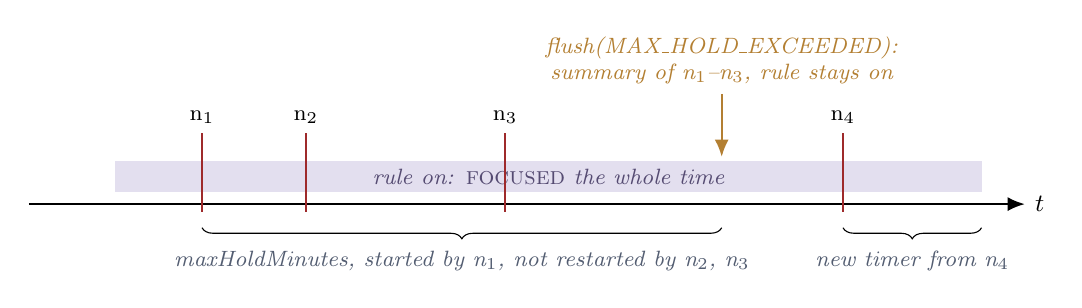
\begin{tikzpicture}[font=\small,x=1.1cm]
  \draw[->,thick](0,0)--(11.5,0) node[right]{$t$};
  \fill[wc!25](1,0.15)rectangle(11,0.55);
  \node[note,text=wc!60!black] at (6,0.35){rule on: \state{focused} the whole time};
  \foreach \x/\l in {2/n$_1$,3.2/n$_2$,5.5/n$_3$,9.4/n$_4$}{
    \draw[thick,rust](\x,-0.1)--(\x,0.9); \node[above,font=\footnotesize] at (\x,0.9){\l};}
  \draw[decorate,decoration={brace,mirror,amplitude=4pt}](2,-0.3)--(8,-0.3)
    node[midway,below=5pt,note]{maxHoldMinutes, started by n$_1$, not restarted by n$_2$, n$_3$};
  \draw[thick,amber!80!black,->](8,1.4)--(8,0.6); \node[above,note,text=amber!80!black] at (8,1.4){flush(MAX\_HOLD\_EXCEEDED):\\summary of n$_1$--n$_3$, rule stays on};
  \draw[decorate,decoration={brace,mirror,amplitude=4pt}](9.4,-0.3)--(11,-0.3)
    node[midway,below=5pt,note]{new timer from n$_4$};
\end{tikzpicture}
\caption{The max-hold safety valve. The timer measures the oldest held item, so a steady trickle of
arrivals cannot keep the first one hidden indefinitely.}\label{fig:maxhold}
\end{figure}

\subsection{Do Not Disturb: \code{DndController}}

The app owns exactly one \code{AutomaticZenRule}, named ``Focus Mode'', identified by the
condition URI \code{condition://com.example.compx551a4/focus}. Switching focus on and off never
adds or removes the rule; it calls \code{setAutomaticZenRuleState} with a \code{Condition} whose
state is \code{STATE\_TRUE} or \code{STATE\_FALSE}. The rule's interruption filter is always
\code{INTERRUPTION\_FILTER\_PRIORITY}, which means ``only what the rule's \code{ZenPolicy} allows''.

Three things about \code{ensureRule} (\file{DndController.kt:76}) are worth being able to explain:

\begin{enumerate}
\item It is \textbf{lazy}. The container is built in \code{Application.onCreate}, before onboarding
  has granted notification-policy access, so registering in the constructor would fail.
\item It \textbf{reuses} an existing rule. It scans \code{automaticZenRules} for one whose
  \code{conditionId} matches before adding; the earlier version added a new rule on every launch.
\item Every platform call is inside \code{runCatching}, and without policy access the method logs
  and returns. This is the fail-open behaviour \file{DESIGN.md}~\S3 demands: no access, no
  suppression, notifications arrive normally.
\end{enumerate}

\begin{why}[Why a zen rule rather than \code{setInterruptionFilter()}]
A rule is the platform's intended API for app-driven DND. It composes with the user's other rules,
appears in system Settings under schedules (where tapping it opens \code{MainActivity}, which is
why the manifest carries the \code{AUTOMATIC\_ZEN\_RULE} intent filter), carries its own
\code{ZenPolicy} for the breakthrough list, and the system restores the previous state when the
rule turns off. A global filter call would overwrite whatever DND the user had set.
\end{why}

\paragraph{\code{BreakthroughPolicy}} is a stateless \code{object} with two functions.
\code{zenPolicyFor(settings)} (API~29+) starts from \code{disallowAllSounds()} and re-allows
selectively, so each \code{PolicySettings} toggle maps one-to-one onto the platform
(\cref{tab:zen}). \code{isBreakthrough(n, settings)} is the listener-side classification: true for
an allow-listed package, or for category \code{call} when calls are allowed, or category
\code{alarm} when alarms are allowed. Category is the only signal the listener has; starred-contact
and repeat-caller decisions happen inside the system and are invisible to the app.

\begin{table}[htbp]\centering\small
\begin{tabular}{@{}l l@{}}
\toprule
\textbf{PolicySettings} & \textbf{ZenPolicy.Builder call} \\
\midrule
(always) & \code{disallowAllSounds()} first \\
\code{allowAlarms} & \code{allowAlarms(bool)} \\
\code{allowCalls} / \code{allowStarredContacts} & \code{allowCalls(ANYONE / STARRED / NONE)} \\
\code{allowRepeatCallers} & \code{allowRepeatCallers(bool)} \\
\code{allowStarredContacts} & \code{allowMessages(STARRED / NONE)} \\
\code{allowedPackages} & nothing: a DND policy has no per-app allowlist \\
\code{maxHoldMinutes} & nothing: handled by the controller's timer \\
\bottomrule
\end{tabular}
\caption{How \code{BreakthroughPolicy.zenPolicyFor} translates settings. Below API~29 the legacy
rule constructor is used and the system's own Priority settings decide what breaks through.}
\label{tab:zen}
\end{table}

\begin{gotcha}[Known limits to state plainly]
\code{allowedPackages} is flagged in the queue but nothing lets those packages through, and there
is no settings UI for it. The old \code{allowTwoFactorCodes} toggle was removed because nothing
could honour it. A starred-contact call that the platform lets through while \code{allowCalls} is
off is flagged \code{breakthrough = false}. If the service is killed without \code{onDestroy}
running, the rule can stay on until the user turns it off in Settings; the battery-optimisation
exemption in onboarding is the mitigation.
\end{gotcha}

\subsection{Watching the shade: \code{FocusNotificationListener}}

The \code{NotificationListenerService} is instantiated by the system, so it cannot be
constructor-injected; it reaches the controller through \code{FocusApp.container.suppressor}
(\file{FocusNotificationListener.kt:20}). It overrides only \code{onNotificationPosted} and
\code{onNotificationRemoved}, and never calls \code{cancelNotification} or
\code{snoozeNotification}.

\code{isUserFacing} (\file{FocusNotificationListener.kt:53}) drops four kinds of notification
before they reach the queue: the app's own package (otherwise the catch-up summary would queue
itself), ongoing ones (media, navigation, downloads), group summaries (they would duplicate their
children), and foreground-service notifications. Everything else that arrives while
\code{controller.isFocused} becomes a \code{DeferredNotification} keyed on
\code{StatusBarNotification.key}, titled from \code{EXTRA\_TITLE} falling back to
\code{EXTRA\_TEXT}, labelled with the app's display name via \code{PackageManager} (falling back
to the package name), and carrying \code{sbn.notification.category}. Removals forward the key so
dismissed items leave the queue.

The manifest entry is guarded by \code{BIND\_NOTIFICATION\_LISTENER\_SERVICE}, a signature
permission that only the system holds. It protects the service from being bound by other apps; it
is not something the app requests. The user grants access in system Settings, which onboarding
opens with \code{ACTION\_NOTIFICATION\_LISTENER\_SETTINGS} and checks afterwards with
\code{getEnabledListenerPackages}. In \file{PermissionChecks.kt} this access is optional: without
it DND still silences, the queue just stays empty.

\subsection{The queue and the summary}

\code{DeferralQueue} is a \code{@Synchronized} wrapper around a \code{LinkedHashMap} keyed on the
platform notification key, so it is oldest-first and an app that updates a notification in place
(``3 new messages'' becoming ``4'') replaces its entry instead of appearing twice. \code{add}
removes before putting, which moves an updated entry to the newest position. It has no size limit;
the max-hold valve bounds it in practice.

\code{CatchUpNotifier.present} (\file{CatchUpNotifier.kt:30}) builds the one grouped summary:

\begin{itemize}
\item Its own channel \code{catch\_up} at \code{IMPORTANCE\_DEFAULT}, which sounds but never
  shows a heads-up. \file{DESIGN.md} is explicit that a burst of heads-up notifications is a worse
  interruption than the one being prevented.
\item Title ``$n$ notifications while you were focused''. The content line depends on the
  \code{FlushReason}: the distinct app names for \code{FOCUS\_BROKE}, otherwise a short phrase
  such as ``Held for the maximum time'' or ``Headset removed''.
\item \code{InboxStyle} with the seven newest items, newest first, as ``App: title'' lines, and a
  ``$+k$ more'' summary line beyond that.
\item Tapping it opens the stfu launcher activity, not the originating apps; the originals are
  still sitting in the shade because DND only silenced them.
\item Posted under the constant id 2001, so a second flush replaces the previous summary rather
  than stacking. A missing \code{POST\_NOTIFICATIONS} grant raises \code{SecurityException},
  which is caught and logged.
\end{itemize}

\subsection{Settings: \code{NotificationSettings}}

A \code{SharedPreferences} file named \code{notification\_policy}, read once at construction and
written on every change. \code{update} sets the \code{StateFlow} first so the controller and the
settings screen react immediately, then does a synchronous \code{commit()} on \code{Dispatchers.IO}
so the write is durable before the call returns. The controller's \code{init} block collects
\code{policy.settings} and forwards every value to \code{gate.updatePolicy}, which rebuilds the rule
with a fresh \code{ZenPolicy}. The settings screen edits the four booleans and the slider; nothing
edits \code{allowedPackages}.

\subsection{What the tests pin down}

\file{NotificationControllerTest.kt} has nine tests built on fakes for the gate, presenter,
recorder and policy, with \code{runTest} and an unconfined dispatcher so virtual time can be
advanced. Being able to recite them is a good way to be sure of the behaviour: \state{focused}
turns the gate on and anything else turns it off; nothing is held outside \state{focused}; a focus
break releases one summary with reason \code{FOCUS\_BROKE} and the gate is already off when it is
posted; an empty queue flushes silently; an updated notification replaces its entry; a dismissed
one leaves; max hold fires after exactly \code{maxHoldMinutes} with focus mode still on, and a
later arrival starts a fresh timer; breakthrough items are flagged but still listed; and a policy
update reaches the gate exactly once.
% =============================================================================
\section{Workload D: UI, onboarding, calibration tasks and stats}\label{sec:d}
% =============================================================================

\begin{files}
\file{MainActivity.kt}, \file{ui/FocusNavHost.kt}, \file{ui/ViewModelFactories.kt},
\file{ui/model/LiveStatus.kt}, \file{ui/home/HomeScreen.kt}, \file{ui/onboarding/*},
\file{ui/calibration/CalibrationScreen.kt}, \file{ui/calibration/tasks/*},
\file{ui/stats/StatsScreen.kt}, \file{ui/settings/SettingsScreen.kt}, \file{ui/common/*},
\file{ui/theme/*}, \file{ui/preview/*}, \file{data/SessionStore.kt}, \file{data/UiPreferences.kt},
tests under \file{test/.../ui/}
\end{files}

The UI is the largest workload by line count but most of it is ordinary Compose. The parts
that need explaining are the ones where a decision was made for a signal-processing or
fail-open reason rather than a visual one: the start-destination latch, what the home pill shows,
the calibration protocol and its four tasks, and how focused time is measured in the session log.

\subsection{Structure: one activity, five routes, ViewModels with factories}

\code{MainActivity} does three things: \code{setContent} with the app theme and \code{FocusNavHost},
\code{eegSource.hold()} in \code{onResume}, and \code{eegSource.release(keepConnected =
serviceController.running.value)} in \code{onStop} unless a configuration change is in progress.

Every ViewModel takes plain constructor arguments and gets them through a companion
\code{Factory} built with \code{viewModelFactory}. The single DI hook is the
\code{container()} extension in \file{ViewModelFactories.kt}, which casts the
application to \code{FocusApp}. That is why the UI tests need no Android \code{Context}; the test
file header says that if they ever do, something leaked into a ViewModel.

\begin{figure}[htbp]\centering
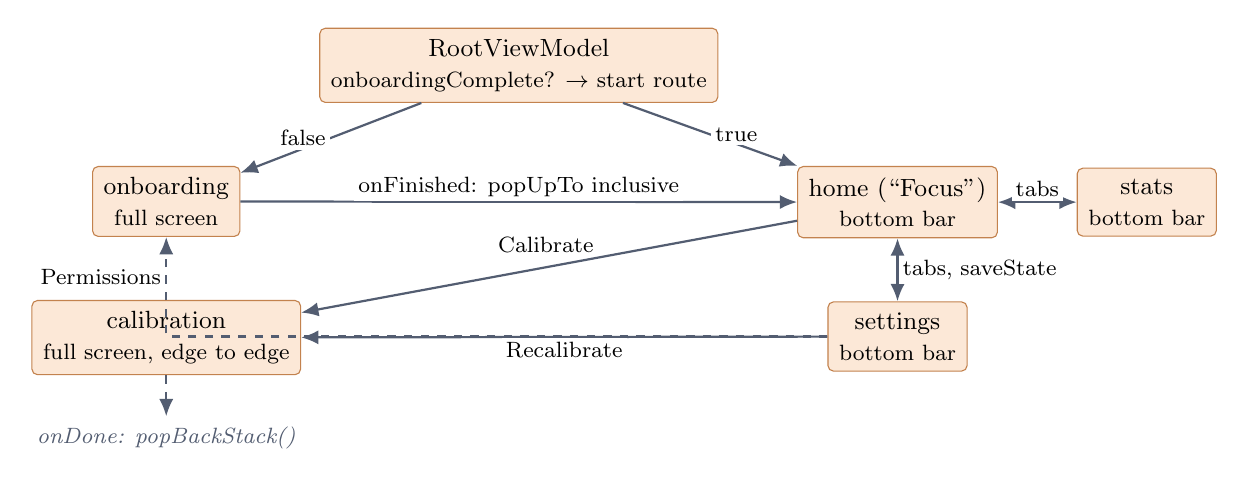
\begin{tikzpicture}[font=\small,node distance=8mm and 10mm]
  \node[wdbox](root){RootViewModel\\\footnotesize onboardingComplete? $\to$ start route};
  \node[wdbox,below left=of root](ob){onboarding\\\footnotesize full screen};
  \node[wdbox,below right=of root](home){home (``Focus'')\\\footnotesize bottom bar};
  \node[wdbox,right=of home](stats){stats\\\footnotesize bottom bar};
  \node[wdbox,below=of home](set){settings\\\footnotesize bottom bar};
  \node[wdbox,below=of ob](cal){calibration\\\footnotesize full screen, edge to edge};
  \draw[flow](root)--(ob) node[midway,left,lbl]{false};
  \draw[flow](root)--(home) node[midway,right,lbl]{true};
  \draw[flow](ob)--(home) node[midway,above,lbl]{onFinished: popUpTo inclusive};
  \draw[flow,<->](home)--(stats) node[midway,above,lbl]{tabs};
  \draw[flow,<->](home)--(set) node[midway,right,lbl]{tabs, saveState};
  \draw[flow](home)--(cal) node[pos=0.4,above left,lbl]{Calibrate};
  \draw[flow](set)--(cal) node[midway,below,lbl]{Recalibrate};
  \draw[flow,dashed](set.west)-|(ob.south) node[pos=0.8,left,lbl]{Permissions};
  \draw[flow,dashed](cal)--++(0,-1.0) node[below,note]{onDone: popBackStack()};
\end{tikzpicture}
\caption{The navigation graph in \file{ui/FocusNavHost.kt}. Routes are plain strings; the graph
has five destinations and no arguments, so type-safe routes were not worth the serialization
plugin.}\label{fig:nav}
\end{figure}

\begin{why}[Why the start destination is latched]
\code{RootViewModel} maps the onboarding preference to a start route, with \code{null} meaning
``not read yet''. The host renders an empty box until it is known, otherwise the user would land
on Home and be yanked to Onboarding a frame later. Once known, the value is latched in
\code{rememberSaveable}, because finishing onboarding flips the preference and letting that reach
\code{startDestination} would rebuild the whole graph under the user. Insets are applied per
destination rather than on the \code{NavHost} because calibration must paint edge to edge.
\end{why}

\subsection{\code{LiveStatus} and the home screen}

\code{liveStatusFlow} in \file{ui/model/LiveStatus.kt} combines the device status, the
\emph{applied} state from the \code{ServiceController}, the thresholds, the recalibration flag,
the deferred list and the running flag into one \code{LiveStatus}, shared by the home and
calibration ViewModels. Its derived \code{signalTrustworthy} is \code{device.usable \&\&
contact.worst <= 2}.

\code{HomeViewModel} runs three collectors: the live status (tracking when the focus state last
changed), the engine's decisions (kept as the last \code{CHART\_WINDOW = 120} \code{FocusPoint}s,
two minutes at 1\,Hz), and an injected one-second ticker that updates the ``for 14m\,12s'' text.
The ticker is injected so tests can pass \code{emptyFlow()}; a \code{delay} loop inside the
ViewModel would hang every test on the virtual clock. Permissions are re-read on every
\code{ON\_RESUME} because special access can be revoked in system Settings while the screen is
stopped.

Two derived rules decide what the master switch does. \code{blocker} is
\code{PERMISSIONS\_MISSING} if any required permission is absent, else \code{NOT\_CALIBRATED} if
there are no thresholds, else null; and \code{canToggle = serviceRunning || blocker == null}, so a
running service can always be turned off. The switch calls \code{serviceController.start()} or
\code{stop()}; a ``release now'' button calls \code{suppressor.flush(MANUAL)}.

The screen is four cards: the switch with a \code{StatusPill}; the signal card with
\code{FocusIndexChart}; the device card with \code{ContactQualityMeter}, battery and a contact
hint; and the deferred card, which lists ``App $\cdot$ count'' and never message content, because
reading the messages here would be the same interruption the app exists to prevent.

\paragraph{The chart} (\file{ui/common/Charts.kt}) is a hand-drawn \code{Canvas}, not a library.
Its y-range is a fixed $\pm3$\,SD, widened only if the signal leaves it, because auto-scaling would
make a calm and a volatile signal look identical. Its x-axis is sized to the \emph{capacity} of 120
slots, so after a screen re-creation new points enter from the right at one per second instead of
stretching and then squeezing. Rejected epochs break the polyline, since interpolating over
discarded data would misrepresent the one thing the chart shows. The hysteresis band between
$\Thigh$ and $\Tlow$ is shaded with dashed guides.

\subsection{Onboarding}

Five steps, in \code{PermissionStepId} order: notifications, Bluetooth, listener, DND, battery.
Only Bluetooth and DND are marked \code{required}; the listener is optional because without it
DND still silences, you merely get no queue. Each step has a detection rule and a request route
(\cref{tab:onboarding}). Results from the launchers are ignored on purpose, and everything is
re-read on resume: a denied dialog and a dismissed one are indistinguishable, and the three
special-access pages return no result at all. The single footer button reads ``Continue'' once
the required steps are granted and ``Skip for now'' otherwise; leaving without grants is allowed
because fail-open applies to setup too.

\begin{table}[htbp]\centering\footnotesize
\begin{tabularx}{\textwidth}{@{}l l X X@{}}
\toprule
\textbf{Step} & \textbf{Required} & \textbf{Detected by} & \textbf{Requested by} \\
\midrule
Notifications & no & \code{checkSelfPermission} & \code{POST\_NOTIFICATIONS} dialog on 33+, nothing below \\
Bluetooth & yes & \code{checkSelfPermission} & \code{BLUETOOTH\_SCAN} + \code{CONNECT} on 31+, \code{ACCESS\_FINE\_LOCATION} below \\
Listener & no & \code{getEnabledListenerPackages} & \code{ACTION\_NOTIFICATION\_\allowbreak LISTENER\_SETTINGS} \\
DND & yes & \code{isNotificationPolicyAccessGranted} & \code{ACTION\_NOTIFICATION\_\allowbreak POLICY\_ACCESS\_\allowbreak SETTINGS} \\
Battery & no & \code{isIgnoringBatteryOptimizations} & direct request with \code{package:} URI, falling back to the list page on OEMs that refuse it \\
\bottomrule
\end{tabularx}
\caption{The onboarding steps in \file{ui/onboarding/PermissionChecks.kt}.}\label{tab:onboarding}
\end{table}

\subsection{The calibration screen and its tasks}\label{sec:d:calibration}

\code{CalibrationViewModel} (\file{CalibrationScreen.kt:127}) is a small state machine over the
sealed \code{CalPhase}, whose cases are Intro, Blocked, Baseline, Countdown, Running, Question,
Rest, Fitting and Done. \code{runProtocol()}
(\file{CalibrationScreen.kt:203}) drives it as in \cref{fig:protocol}.

\begin{figure}[htbp]\centering
\resizebox{\textwidth}{!}{%
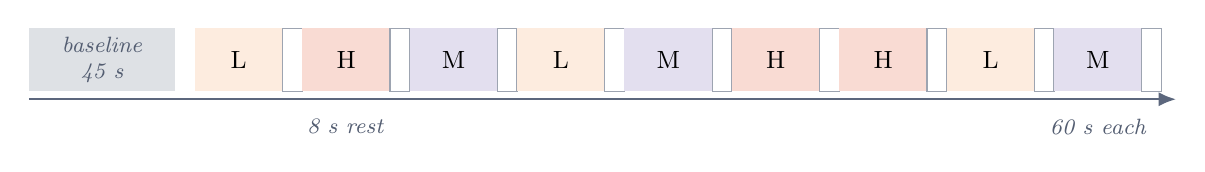
\begin{tikzpicture}[font=\small,x=0.62cm]
  \fill[slate!20](0,0)rectangle(3,0.8); \node[note] at (1.5,0.4){baseline\\45 s};
  \foreach \i/\c/\col in {0/L/wd!20,1/H/wb!25,2/M/wc!25,3/L/wd!20,4/M/wc!25,5/H/wb!25,6/H/wb!25,7/L/wd!20,8/M/wc!25}{
    \pgfmathsetmacro{\x}{3.4+\i*2.2}
    \fill[\col](\x,0)rectangle(\x+1.8,0.8); \node[font=\small] at (\x+0.9,0.4){\c};
    \draw[slate!60](\x+1.8,0)rectangle(\x+2.2,0.8);
  }
  \node[note] at (3.4+8*2.2+0.9,-0.45){60 s each};
  \node[note] at (3.4+0.9*2.2+1.1,-0.45){8 s rest};
  \draw[->,thick,slate](0,-0.1)--(23.5,-0.1);
\end{tikzpicture}}
\caption{One calibration run, about nine minutes. \textsc{l}, \textsc{m}, \textsc{h} are the
\code{LOW}, \code{MEDIUM} and \code{HIGH} conditions, three of each in an order shuffled per run.
Before each block the screen waits for a trustworthy signal and counts down from 5. A \code{MEDIUM}
block is followed by one comprehension question. A block with under 50\,\% valid epochs is discarded
and its condition re-queued, at most three times. Fast mode (a developer toggle) uses 6\,s blocks,
a 4\,s baseline, 1.5\,s rests, and 600\,ms 2-back items.}\label{fig:protocol}
\end{figure}

Points that matter for the fit, all with a comment in the code:
\begin{itemize}
\item The source is started by the ViewModel only if no session is running, and
  \code{focusEngine.reset()} precedes the baseline. All epochs are captured into one list while
  \code{recording} is true; blocks are matched to them later by timestamp.
\item Block order is shuffled so a time-into-session effect (fatigue, drying gel, a settling
  headband) cannot masquerade as a condition effect.
\item The reading question is asked \emph{after} recording stops, because answering is a different
  task and its epochs would be mislabelled \code{MEDIUM}. Only reading blocks can end early, via
  ``Finished'': a finished reader is just waiting. ``Not sure'' answers null and scores 0 of 1,
  which B then drops as low accuracy.
\item \code{awaitUsableSignal()} only blocks \emph{between} blocks, the one moment the user can fix
  the headband without disturbing a recording.
\item \code{accept()} calls \code{updateThresholds} only if the engine's current thresholds differ
  from the result's, so a separable fit (already applied by the engine) and an unfitted result
  (which returns the thresholds already in use) both change nothing.
\end{itemize}

\paragraph{Matched visual input.} Every task renders inside \code{TaskScaffold}: the same dark
\code{CalibrationTaskTheme} regardless of system theme, the instruction in a fixed 56\,dp slot, the
task centred in the remaining space, the block label and countdown at the bottom. \file{DESIGN.md}~\S2
requires eyes open with matched visual input across conditions; without it the comparison
measures screen brightness as much as cognition. For the same reason the screen holds
\code{FLAG\_KEEP\_SCREEN\_ON} and serial subtraction uses an on-screen keypad rather than the IME.

\begin{table}[htbp]\centering\small
\begin{tabularx}{\textwidth}{@{}l l X l@{}}
\toprule
\textbf{Task} & \textbf{Condition} & \textbf{What happens} & \textbf{Score} \\
\midrule
\code{FixationTask} & \code{LOW}, baseline & A 7\,dp dot drifting round a circle, one lap per 20\,s,
  driven by \code{withFrameNanos} so it still moves with animator scale off. A moving dot holds the
  gaze and discourages slow blinks. & none \\
\code{ReadingTask} & \code{MEDIUM} & One of three passages, rotated between runs so a repeat is not a
  memory test, plus ``Finished''. Then \code{ReadingQuestion} with three options and ``not sure''. &
  0 or 1 of 1 \\
\code{NBackTask} & \code{HIGH} & 2-back over nine consonants, 1.5\,s per item, 30\,\% targets, never
  the same letter twice in a row. Hits and correct rejections count as correct; false alarms and
  reaction times are recorded. & correct / scored \\
\code{SerialSubtractionTask} & \code{HIGH} & Count down in sevens from a random 500--999 on a 4$\times$3
  keypad. No right/wrong feedback (an error signal is itself a cognitive event), and the next prompt
  continues from the true value so one slip does not poison the block. & correct / attempts \\
\bottomrule
\end{tabularx}
\caption{The calibration tasks in \file{ui/calibration/tasks/}. The user picks which
\code{HIGH} task to use in Settings.}\label{tab:tasks}
\end{table}

\begin{gotcha}[Two engagement-check weaknesses to know]
Because correct non-responses count, a user who never presses MATCH still scores roughly the
non-target rate, about 60--70\,\%, which passes B's 50\,\% threshold; the check is strongest against
random pressing. And a single reading question decides each \code{MEDIUM} block, so one wrong
answer drops it. Both are open questions in \file{SUMMARY\_B.md}.
\end{gotcha}

\paragraph{The result screen} distinguishes three outcomes. \code{fitted = false} shows ``Not
enough clean data'', a dash where the AUC would be (a 0.50 would read as a measured chance result),
and offers ``Redo'' or ``Keep current thresholds''. A fitted result shows the AUC in large type with
a verdict (good at $\ge 0.75$, fair at $\ge 0.60$, otherwise ``barely better than chance'', worded
as a finding about consumer EEG rather than user error), a \code{SeparationBar} of the two class
means, the thresholds, and the pooled task accuracy, then ``Use these thresholds'' or ``Redo''.

\subsection{Stats, settings, theme}

\paragraph{Stats} is \code{SessionStats} rendered directly: four \code{StatTile}s (total focus,
longest streak, deferred, delivered), a \code{TimeOfDayChart} of 24 bars where every hour keeps a
2\,dp sliver so zero reads as zero rather than a gap, and a history list. There are no queries; all
aggregates are getters over the in-memory session list.

\paragraph{Settings} writes to three different stores, which is the thing to be clear about
(\cref{tab:settings}). The dwell sliders are hidden until thresholds exist, because showing them
would write placeholder values the user would mistake for their own. ``Load placeholder
thresholds'' is the developer escape hatch that skips calibration.

\begin{table}[htbp]\centering\small
\begin{tabularx}{\textwidth}{@{}l l X@{}}
\toprule
\textbf{Setting} & \textbf{Range} & \textbf{Written through} \\
\midrule
Exit timeout, entry dwell & 10--300\,s, 3--60\,s & \code{FocusEngine.updateThresholds} $\to$ \code{ThresholdStore} (B) \\
Max hold, four allow toggles & 5--120\,min & \code{NotificationPolicy.update} $\to$ \code{NotificationSettings} (C) \\
Fast calibration, high-demand task & & \code{UiPreferences} DataStore \code{ui\_prefs} (D) \\
Placeholder thresholds, clear history & & \code{updateThresholds(PLACEHOLDER)}, \code{SessionStore.clear()} \\
\bottomrule
\end{tabularx}
\caption{Where each setting goes. \code{allowedPackages} has no UI.}\label{tab:settings}
\end{table}

\paragraph{Theme.} A low-chroma teal and slate palette in \file{ui/theme/Color.kt}: the app is
looked at while concentrating, and during calibration it \emph{is} the visual field. Dynamic colour
is off by default so demo screenshots are consistent across devices. Every status colour is paired
with an icon and a label, never used alone. \code{FocusTheme.colors.forHsi()} maps HSI 1 to good,
2 to fair, worse to poor, which is what the contact meter draws.

\subsection{\code{SessionStore}: the session log}

\code{SessionStore} implements \code{SessionRecorder} with an append-only \code{sessions.jsonl}
in \code{filesDir}, one line per completed session, written once at \code{onSessionEnd}. Decisions
arrive at 1\,Hz and are accumulated in memory; there is no per-decision I/O. Focused time is
measured \emph{between transitions} (a \state{focused} edge starts a streak, the next
non-\state{focused} decision closes it), not by counting \state{focused} decisions, so a dropped or
rejected epoch cannot silently shorten the total. Each closed streak is split across hour
boundaries with \code{Calendar} in local time into the 24-slot \code{focusedMsByHour}, so a streak
over midnight lands in the right buckets. \code{onDeferred} and \code{onFlush} just count. A session
with no focused time and nothing deferred is discarded rather than logged. Reading tolerates a
truncated last line: a crash mid-append should cost one session, not the history. There is no
retention limit; only the developer ``clear'' deletes the file.

\code{UiPreferences} is a Preferences DataStore named \code{ui\_prefs} holding
\code{onboardingComplete}, \code{highDemandTask} and \code{fastCalibration}. It is deliberately
separate from C's \code{NotificationSettings} and B's \code{ThresholdStore}, which hold domain state.

\subsection{\code{ui/preview}: the demo stack}

\file{DemoStack.kt} holds in-memory stand-ins for A, B and C (\code{DemoEegSource},
\code{DemoFocusEngine}, \code{DemoSuppressor}, \code{DemoServiceController}) written so the UI
could be built and previewed before the real modules existed. Its header says it should be deleted
at integration and that if anything in \code{ui/} has to change when that happens, the contract
boundary was drawn in the wrong place. It is no longer wired into the container, but it remains
for Compose previews and for \file{DemoFocusEngineTest}, whose four tests are written against the
\code{FocusEngine} contract (uncalibrated stays \state{unknown}; one spike does not silence the
phone; clean separation gives AUC 1.0; empty input gives 0.5) and so should pass against B's
pipeline too. \code{DemoFocusEngine} is also a useful 150-line summary of what B's pipeline does,
minus smoothing, the calibration reference, artifact holdoff and drift.
% =============================================================================
\section{Integration: what changed when the branches met}\label{sec:integration}
% =============================================================================

\begin{files}
\file{docs/area\_specific\_changes.md}, \file{MUSE\_CONNECTION\_FIXES.md}, \code{git log} from
\code{3bec20d} to \code{bf5774e}
\end{files}

The four branches were merged on 3 October and tested on a Galaxy S23 Ultra with the headband
\code{Muse-3973}. Several behaviours changed during that afternoon, and some of the per-workload
documents (\file{SUMMARY\_B.md} in particular) predate them. If you own one of these areas, the
version in \code{main} is the one to describe. \Cref{tab:integration} is the list; the reasons are
in the sections above where they belong.

\begin{table}[htbp]\centering\small
\begin{tabularx}{\textwidth}{@{}l X X@{}}
\toprule
\textbf{Area} & \textbf{Change} & \textbf{Observed cause} \\
\midrule
A & 10\,s signal-loss grace, then flush as \code{HEADSET\_REMOVED}, apply \state{unknown}, reset the
  engine; session ends itself after 120\,s without signal; \code{appliedState} published. &
  One electrode at HSI~2 for four seconds released the whole queue and toggled DND twice. \\
A & \code{start()} refuses to mark itself started without BLE permission; no contact state or
  epochs until \code{linkUp}; stale-advertisement rule and 1\,s list polling after a drop;
  \code{hold()} moved to \code{onResume}. & A switched-off headband cycled Disconnected and Poor
  contact; a launch before onboarding never scanned again. \\
A & \code{watchForHeadsetRemoved()} deleted. & It counted \code{StateFlow} emissions, which only
  happen on change. \\
A & \code{runDecisionLoop()} became a \code{coroutineScope} block so its collectors are children of
  \code{loopJob}. & Found while writing this guide: the collectors were siblings on the service scope
  and survived \code{onDestroy}. \\
B & \code{FocusPipeline} gained \code{smoothingWindow} (container passes 8) and
  \code{useCalibrationReference} (default on); \code{RollingZScore.score()} added;
  \code{Insufficient} now returns \code{fitted = false}. B's own tests pass unchanged; five
  smoothing tests added. & With a real fit of $+0.23 / +0.07$ the longest run above $\Thigh$ in
  11 minutes was 8\,s; the rolling window normalised long focus away. \\
C & Everything rewritten so it runs: lazy, reusable zen rule with a \code{ZenPolicy};
  \code{FocusModeGate} and \code{CatchUpPresenter} seams; max-hold timer; one \code{InboxStyle}
  summary; listener filters; keyed queue; \code{SharedPreferences} settings; nine unit tests. &
  The merged code had an unassigned \code{lateinit}, registered the rule before access existed,
  an empty settings file and a TODO where the summary should be. \\
D & ``Use these thresholds'' applies the shown values; 2-back never repeats a letter and runs at
  1.5\,s; reading has ``Finished''; fixation dot on the frame clock; ``Not enough clean data''
  result; chart x-axis fixed at 120\,s; pill shows \code{appliedState}; dead switches removed. &
  Animations off in Developer options froze the dot; fast calibration always returned
  \code{Insufficient}. \\
Shared & \code{ServiceController.appliedState} added; \code{DeferredNotification.category} and
  \code{CalibrationResult.fitted} added; \code{allowTwoFactorCodes} removed; app renamed
  \textsc{stfu}. & \\
\bottomrule
\end{tabularx}
\caption{Integration changes by area. The source for this table is
\file{docs/area\_specific\_changes.md}.}\label{tab:integration}
\end{table}

\paragraph{Evidence the signal path works.} Replaying the 620 epochs logged during an 11-minute
reading session through the live rules, with that user's fitted thresholds, gave:

\begin{center}\small
\begin{tabular}{@{}l r@{}}
\toprule
\textbf{Normalisation} & \textbf{Time \state{focused}} \\
\midrule
Rolling window, no smoothing & 0\,\% \\
Calibration reference, no smoothing & 87\,\% \\
Calibration reference, 8-epoch smoothing & 98\,\% \\
\bottomrule
\end{tabular}
\end{center}

Live afterwards: reading gave a smoothed $z$ of about $+0.4$; counting backwards from 300 in
sevens gave $+2.0$ with every sample above $\Thigh$; idly looking at the screen gave $+0.1$, inside
the dead band, and the state stayed \state{not\_focused}. All three match what the user was doing.

\paragraph{Open decisions the team has not made.} Whether the calibration reference should drift
slowly (a long EMA) rather than stay fixed until recalibration; whether the muscle ratio of 1.3
rejects real focus; who owns artifact flagging, A's source or B's rejector; and the
engagement-check gaps on the 2-back and the single reading question.

\subsection{Test inventory}

\begin{table}[htbp]\centering\small
\begin{tabularx}{\textwidth}{@{}l l X@{}}
\toprule
\textbf{Area} & \textbf{Test file} & \textbf{What it pins down} \\
\midrule
B & \file{FocusStateMachineTest} & dwell timing, dead band, no chatter, gap restart, live threshold edit \\
B & \file{ArtifactRejectorTest} & the five reasons in order, 2\,s inclusive holdoff, relative muscle rule \\
B & \file{FocusPipelineTest} & warm-up, acceptance flags, reset; \code{RollingZScore} semantics \\
B & \file{FocusPipelineSmoothingTest} & the real fit $0.23/0.07$ is only reachable with smoothing \\
B & \file{FocusPipelineCalibrationTest} & apply only if separable, history always, startup load \\
B & \file{DriftDetectorTest} & shift and spread rules, sustain count, prompt latches \\
B & \file{CalibrationSessionTest}, \file{\ldots SettleTest} & drop reasons, settle, holdoff across blocks \\
B & \file{ThresholdFitterTest} & hysteresis geometry, scale invariance, AUC ties, insufficient \\
B & \file{ThresholdStoreTest} & round trip, atomic write, corrupt lines, validation \\
C & \file{NotificationControllerTest} & gate on/off, one summary, max hold, dedupe, breakthrough flag \\
D & \file{HomeViewModelTest} & blockers, chart window, gaps, manual release, poor contact \\
D & \file{NBackScoringTest}, \file{FormatTest}, \file{DemoFocusEngineTest} & scoring rules, formatting, engine contract \\
A & none & the device layer is verified on the phone; see \file{MUSE\_CONNECTION\_FIXES.md} \\
\bottomrule
\end{tabularx}
\caption{Unit tests, all plain JUnit under \file{app/src/test}. Run with
\code{./gradlew :app:testDebugUnitTest}.}\label{tab:tests}
\end{table}
% =============================================================================
\section{Question bank}\label{sec:questions}
% =============================================================================

Answer each from memory first, then check it against the section cited. The questions are
ordered roughly from ``anyone on the team should get this'' to ``only the owner would''.
\begin{multicols}{2}\small

\subsection*{Architecture}

\Q{What is the one-sentence description of the app, and which Android mechanism does the
suppression?}{While a Muse EEG headset indicates the wearer is concentrating, hold the phone's
notifications back and deliver them as one quiet summary when concentration breaks. Suppression is
an \code{AutomaticZenRule} (Do Not Disturb in Priority mode), not cancelling or snoozing
(\cref{sec:c}).}

\Q{Name the four original interfaces, who implements each, and the two that were added
later.}{\code{EegSource} (A), \code{FocusEngine} (B), \code{Suppressor} (C),
\code{SessionRecorder} (D). Added: \code{ServiceController} (A) for the master switch and
\code{NotificationPolicy} (C) for the settings surface (\cref{tab:contracts}).}

\Q{Why is there no dependency-injection framework?}{Five singletons do not justify the build cost,
and a container the team can read on one screen is worth more than annotations. \code{FocusApp}
builds one \code{AppContainer}; ViewModels reach it through \code{CreationExtras.container()}.}

\Q{What does \state{unknown} mean and what must every consumer do with it?}{No usable signal:
headset off, disconnected or not settled. Every consumer fails open: the suppressor turns the rule
off and flushes, the home pill shows ``no signal'', and notifications are delivered normally.}

\Q{Why are thresholds stored as z-scores rather than raw band power?}{Absolute band power drifts
with placement, hair, moisture, headband tension, time of day and caffeine; a raw number calibrated
on Tuesday is wrong on Thursday. z-scores are relative to a distribution, and supplying the right
distribution becomes the pipeline's job.}

\Q{Which thread do LibMuse callbacks arrive on, and where does the decision loop run?}{LibMuse
calls back on the main thread; the decision loop runs in \code{FocusService}'s
\code{SupervisorJob + Dispatchers.Default} scope. Disk writes hop to \code{Dispatchers.IO}
(\cref{fig:threads}).}

\Q{Why does the home screen show \code{appliedState} rather than \code{FocusEngine.state}?}{They
differ during the 10\,s signal-loss grace period and when no session runs; the pill must agree
with what the DND rule is actually doing.}

\subsection*{Workload A}

\Q{Why did the headband never appear at first, and what was the fix?}{The scan permission
lacked the \code{neverForLocation} flag; on Android~12+ scan results are then dropped
unless fine location is held, which was capped at SDK~30. One manifest attribute fixed it.}

\Q{Why does \code{MuseEegSource} poll the manager\textquotesingle s list every second instead of waiting for
the list-changed callback?}{LibMuse only fires the callback for a headband it has never seen; a
known one is silently rediscovered. After a drop or restart the callback never comes.}

\Q{What is \code{staleDiscoveredTime} for?}{After a drop LibMuse lists the headband for about
30\,s with its old discovery time; connecting to that entry while the headband is off just times
out. Only an entry rediscovered after the drop is really advertising.}

\Q{Explain \code{mergeFresh}.}{LibMuse sends \code{NaN} per channel until its first clean window
and then repeats the last clean value while rejecting the current one. Keeping only values that
are finite and changed since the previous packet stops stale values posing as fresh data and one
\code{NaN} channel poisoning the mean. First focus value in about 1\,s instead of 90.}

\Q{Why does \code{average()} return \code{NaN} rather than 0 for an empty channel list?}{Zero
produced a plausible finite index from missing data; \code{NaN} fails
\code{engagementIndex.isFinite()} and the epoch is marked invalid.}

\Q{What are the two drop detectors and the reconnect timing?}{LibMuse's \code{DISCONNECTED}
callback and a watchdog that treats 5\,s of packet silence while connected as a drop. Both call
\code{rescanAfterDrop()} with a 2\,s delay. The service's own backoff runs 2, 4, 8, 16, 30\,s.}

\Q{Why does \code{emitEpoch} return early unless \code{linkUp}?}{Deriving state from an empty
horseshoe during a reconnect showed ``Poor contact'' instead of ``Connecting''.}

\Q{What does \code{ForegroundEegSource} do and why does it ignore \code{stop()}?}{It keeps the
headset connected while the app is visible: \code{hold()} on resume, \code{release()} on stop
unless a session is running. Calibration and the service both call \code{stop()} when they finish;
honouring it would drop the headset with the app open.}

\Q{Why is the service's \code{foregroundServiceType} \code{connectedDevice}, and how does the
UI know whether the service is alive?}{Android~14+ requires a typed foreground service with the
matching permission; a BLE headset is a connected device. The service is unbound; the UI observes
companion \code{StateFlow}s via \code{AndroidServiceController}, which reset if the process dies.}

\Q{Walk through what happens when the headset is taken off mid-session.}{Contact degrades, status
leaves \textsc{connected}; after 10\,s of unusable signal the effective state becomes
\state{unknown}: flush as \code{HEADSET\_REMOVED}, \code{apply(UNKNOWN)} turns the rule off,
\code{focusEngine.reset()}. Backoff reconnects keep trying; after 120\,s the service calls
\code{stopSelf()}, which flushes \code{SERVICE\_STOPPED} and ends the session.}

\Q{Why did the old \code{watchForHeadsetRemoved()} never fire?}{It counted consecutive emissions
of a \code{StateFlow}, which only emits on change, so it never counted five of anything.}

\Q{Why is \code{runDecisionLoop} a \code{coroutineScope} block, and what went wrong before it
was?}{So its collectors are children of \code{loopJob} and die with it in \code{onDestroy}. They
used to be launched on the service scope as siblings, so cancelling the loop job cancelled nothing
and a stopped session kept driving the engine and \code{appliedState} (\cref{sec:a}).}

\Q{Can the \code{emgBroadband} artifact flag fire on the Muse source?}{Effectively no. LibMuse's
relative band powers are fractions in $[0,1]$ and the thresholds are 3.0.}

\subsection*{Workload B}

\Q{Write down the focus index and say where each band comes from.}{Pope et al.\ (1995)
engagement index $\beta/(\alpha+\theta)$. Alpha from the temporal pair TP9/TP10 (less eye
contamination), beta nominally 13--20\,Hz (above that is forehead muscle), theta over all
channels.}

\Q{List the rejector's checks in order and the holdoff rule.}{Source invalid, poor contact (any HSI
$>1$), non-finite, muscle ($\beta > 1.3\times$ the median of the last 60 clean betas, after 10),
holdoff (within 2\,s inclusive of a rejection). A primary rejection restarts the holdoff; a holdoff
rejection does not extend it.}

\Q{Why do muscle-rejected epochs still enter the median window?}{Otherwise a genuine lasting rise
in beta would lock the gate forever. A brief clench cannot move a one-minute median; a lasting
shift is absorbed.}

\Q{Explain the Schmitt trigger with dwell, including what a dead-band value does.}{Above $\Thigh$
starts an entry run; below $\Tlow$ starts an exit run; in between cancels both runs but keeps the
state. Transition when a run has lasted the dwell, measured between timestamps. Defaults $N=10$\,s,
$M=60$\,s; first usable sample goes to \state{not\_focused} (fail open); a gap over 5\,s restarts
runs.}

\Q{At 1\,Hz, how many samples does a 5\,s dwell take, and why?}{Six. The run starts at the first
qualifying sample ($t=0$) and \code{now - start >= 5} is first true at $t=5$.}

\Q{Describe the two normalisation paths and which one is live.}{With a calibration reference,
$z = (\text{smoothed} - \mu_{\text{cal}})/\sigma_{\text{cal}}$. Without one, the rolling z-score
over the last 600 raw values after a 30-sample warm-up. The reference path is live by default
because a rolling window re-centres on a long focus period and normalises it away.}

\Q{Why is the rolling window fed the raw index when the state machine sees the smoothed one?}
{Smoothing shrinks the SD; a smoothed window compared against the calibration reference would
look like spread drift. The window exists for the drift detector and as the fallback.}

\Q{Why 8-epoch smoothing, and what is the evidence?}{A single noisy dip resets the entry run, so
``sustained above $\Thigh$'' was unreachable: the longest run in 11 minutes of real reading was
8\,s. Replaying 620 epochs: 0\,\% focused with the rolling window, 87\,\% with the reference, 98\,\%
with reference plus smoothing.}

\Q{When does the drift detector suggest recalibration?}{Reference present and matching
\code{fittedAtMs}, at least 300 window samples, and for 120 consecutive checks either the mean has
shifted more than one reference SD or the SD ratio is above 2 or below $\tfrac12$. The pipeline
latches the prompt until a separable calibration.}

\Q{What does \code{CalibrationSession.prepare} drop or discard?}{\code{MEDIUM}/\code{HIGH} blocks
with no score, zero attempts or accuracy below 0.5 (never \code{LOW}); the first
$\min(5\,\text{s}, \text{duration}/12)$ of each block; and everything a single fresh
\code{ArtifactRejector} rejects across the whole recording in time order.}

\Q{How are the thresholds placed, and how is AUC computed?}{z-score the whole run (\code{MEDIUM}
included), take the \code{LOW} and \code{HIGH} class means, put the midpoint between them, and set
$\Thigh,\Tlow = m \pm \max(0.15\,d, 0.05)$ where $d$ is the separation. AUC is Mann--Whitney: the
fraction of (high, low) pairs where high scores higher, ties counting half.}

\Q{What is the difference between a non-separable and an insufficient fit, and what does each do?}
{Insufficient: fewer than 10 usable \code{LOW} or \code{HIGH} samples; nothing saved,
\code{fitted = false}, screen says ``not enough clean data''. Non-separable: AUC $< 0.6$ or
\code{HIGH} below \code{LOW}; appended to history as a finding but not applied; thresholds in
use unchanged.}

\Q{How does \code{ThresholdStore} persist, and why not JSON?}{Two \code{key=value;} text files,
\code{current.txt} (temp-and-rename) and append-only \code{history.txt}, under a mutex on
\code{Dispatchers.IO}. \code{org.json} is a stub on the local JVM, and the format is testable
without Robolectric and tolerant of unknown keys.}

\Q{Why does \code{updateThresholds} save before applying, and why does \code{reset()} keep
\code{recalibrationSuggested}?}{Saving first lets the store's validation refuse an invalid set
before it is half-applied. The stale thresholds are still the ones in use next session, so the
prompt should stay up until a successful calibration.}

\subsection*{Workload C}

\Q{Does the app cancel, snooze or re-post notifications?}{No. It toggles one zen rule, watches
the shade with a log-only listener, and posts one summary of its own. Snooze is the unbuilt v2;
cancel-and-repost is impossible because an app cannot post on behalf of another package.}

\Q{Why a zen rule and not \code{setInterruptionFilter()}?}{The rule composes with the user's own
DND, is visible in Settings, carries its own \code{ZenPolicy} for the breakthrough list, and the
system restores the previous state when it turns off. The global call would clobber the user's
settings.}

\Q{Why is the rule created lazily, and why search for an existing one?}{The container is built
before onboarding grants policy access; the earlier code added a new rule on every launch.}

\Q{What does \code{apply()} do for each state, and why in that order?}{\state{focused}: gate on.
Anything else: gate off, then \code{flush(FOCUS\_BROKE)} if the queue is non-empty, so the summary
is posted after the rule is off and is not silenced by it.}

\Q{Describe the max-hold valve precisely.}{A \code{delay(maxHoldMinutes * 60\_000)} started when
the queue goes from empty to non-empty, not restarted by later arrivals, cancelled if the queue
empties. It flushes with \code{MAX\_HOLD\_EXCEEDED} and leaves focus mode on. Default 30~min,
slider 5--120, zero disables.}

\Q{Which notifications never enter the queue?}{The app's own package, ongoing ones, group
summaries, and foreground-service notifications. Anything else while \code{isFocused}, keyed on
\code{sbn.key} so an in-place update replaces its entry.}

\Q{How is the breakthrough list enforced, and what can the app actually see?}{The platform
enforces it through the rule's \code{ZenPolicy} (\code{disallowAllSounds} then re-allow alarms,
calls, repeat callers, starred messages). The listener only sees \code{Notification.category},
so it flags calls and alarms; starred-contact and repeat-caller decisions are invisible to it.
\code{allowedPackages} is flagged but not enforced.}

\Q{Describe the catch-up summary.}{One \code{InboxStyle} notification on channel \code{catch\_up}
at \code{IMPORTANCE\_DEFAULT} (sound, no heads-up), title ``$n$ notifications while you were
focused'', subtitle from the flush reason, seven newest lines, ``$+k$ more'', constant id 2001 so
it replaces itself, tapping opens the app.}

\Q{What is the role of \code{BIND\_NOTIFICATION\_LISTENER\_SERVICE}?}{A signature permission on
the listener's manifest entry so only the system can bind it. The user grants listener access in
Settings; the app never requests this permission.}

\subsection*{Workload D}

\Q{Why does \code{FocusNavHost} latch the start destination and render nothing until it is
known?}{The onboarding preference is read asynchronously; building the graph early would flash
Home then Onboarding, and letting the flipped preference reach \code{startDestination} after
onboarding would rebuild the graph under the user.}

\Q{When can the master switch be toggled?}{\code{canToggle = serviceRunning || blocker == null},
where the blocker is missing required permissions (wins) or no thresholds. A running service can
always be turned off.}

\Q{Why is the one-second ticker injected into \code{HomeViewModel}?}{A \code{delay} loop inside
the ViewModel would hang every test on the virtual clock; tests pass \code{emptyFlow()}.}

\Q{Three design choices in the live chart and the reason for each.}{Fixed $\pm3$\,SD range so calm
and volatile signals look different; x-axis sized to the 120-slot capacity so new points enter from
the right at a steady pace; rejected epochs break the line so discarded data is not interpolated.}

\Q{Which onboarding steps are required, and why can the user skip anyway?}{Bluetooth and DND.
Fail-open applies to setup: a working app that delivers everything beats a dead end. Special-access
pages return no result, so everything is re-read on resume.}

\Q{Describe one calibration run.}{45\,s baseline, then nine 60\,s blocks (three per condition)
in shuffled order with 8\,s rests and a 5\,s countdown each, waiting for a trustworthy signal
between blocks. A \code{MEDIUM} block is followed by one question; a block under 50\,\% valid is
re-queued up to three times. Then \code{fitCalibration} and the result screen.}

\Q{Why is the reading question asked after the block, and why can only reading end early?}
{Answering is a different task whose epochs would be mislabelled \code{MEDIUM}; a finished reader
is just waiting. Stopping fixation or 2-back early would only mean less data.}

\Q{Why does every task use the same dark scaffold and no keyboard?}{\file{DESIGN.md}~\S2 requires
matched visual input across conditions; otherwise the comparison measures brightness and layout
as much as cognition.}

\Q{How does \code{SessionStore} measure focused time, and why?}{Between state transitions, not by
counting \state{focused} decisions, so a dropped or rejected epoch cannot shorten the total. Streaks
are split across hour boundaries into a per-session 24-slot list. Written once per session as a
JSONL line.}

\Q{Where does each settings control write?}{Dwell sliders to the engine and B's
\code{ThresholdStore}; max hold and the four toggles to C's \code{NotificationSettings}; fast
calibration and the task choice to D's DataStore. The dwell sliders are hidden until thresholds
exist.}

\Q{Where would you switch to the fake or OSC source?}{Nowhere in the UI. Edit the one line in
\file{AppContainer.kt}; the demo-mode switch was removed during integration.}
\end{multicols}

\end{document}
